\documentclass{article}
\usepackage{graphicx} % Required for inserting images

\usepackage{amsmath,amssymb,amsfonts}
\usepackage{mathtools}
\DeclarePairedDelimiter\ceil{\lceil}{\rceil}
\usepackage{algorithmic}
\usepackage{graphicx}
\usepackage{textcomp}
\usepackage[acronym,shortcuts]{glossaries}
\usepackage{placeins}
\usepackage{flushend}
\usepackage[utf8]{inputenc}
\usepackage{pgfplots}
\pgfplotsset{compat=newest}
\DeclareUnicodeCharacter{2212}{−}
\usepgfplotslibrary{groupplots,dateplot}
\usetikzlibrary{patterns,shapes.arrows}
\usetikzlibrary{arrows}
\usetikzlibrary{pgfplots.statistics}
\usetikzlibrary{automata, positioning, arrows}
\usetikzlibrary{backgrounds}
\usepackage{mdframed}
\usepackage{lipsum}
\usepackage{booktabs}
\usepackage{siunitx}
\sisetup{per-mode=symbol,per-symbol = p,range-phrase=--, range-units=single,inter-unit-product = {}}
\DeclareSIUnit{\belmilliwatt}{Bm}
\DeclareSIUnit{\dBm}{\deci\belmilliwatt}
\usepackage{float}
%\usepackage[printwatermark]{xwatermark}
\usepackage{pgfplots}
\usepackage{setspace}
\usepackage[font=small]{subcaption}
\usepgfplotslibrary{dateplot} 
\usepackage{eurosym}
\usepackage{tabularx}
\usepackage{nicefrac}
\usepackage{bytefield}
\usepackage{xspace}
\usepackage{soul}

\usepackage{scalerel}
\usepackage{tikz-network}
\usepackage{pgf-umlsd}
\usepackage{tikz-dimline}
\usetikzlibrary{svg.path}
\usetikzlibrary{arrows.meta} 

\newcommand{\multihop}{multi-hop\xspace}
\newcommand{\Multihop}{Multi-hop\xspace}

\title{An Energy-Efficient LoRa Multi-Hop Protocol through
Preamble Sampling for Remote Sensing \\[1ex] \large -- Simulation Results --}
\author{Guus Leenders}
\date{April 2023}

\begin{document}

\maketitle


%%%%%%%%%%%%%%%%%%%%%%%%%%%%%%%%%%%%%%%%%%%%%%%%PAYLOAD SIZE%%%%%%%%%%%%%%%%%%%%%%%%%%%%%%%%%%%%%%%%%%%%%%
\FloatBarrier
\begin{figure}[p]
    \centering
    \include{img/randomaggregation/github_final_simulate_matrix_children_TX_AGGREGATION_TIMER_RANDOM_MEASURE_INTERVAL_S_23_02_22_pdr}
    \vspace{-0.7cm}
    \caption{Simulated packet delivery ratio (PDR) across the \multihop network w.r.t. the added random timer interval ($T_\text{random}$).}
    \label{fig:}
\end{figure}
\begin{figure}[p]
    \centering
    % This file was created with tikzplotlib v0.10.1.
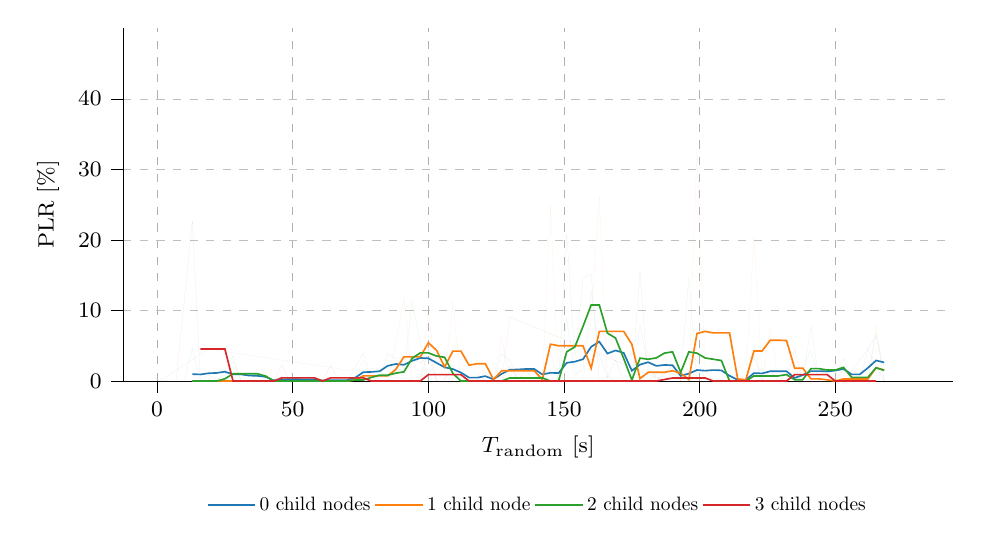
\begin{tikzpicture}

\definecolor{crimson2143940}{RGB}{214,39,40}
\definecolor{darkgray176}{RGB}{176,176,176}
\definecolor{darkorange25512714}{RGB}{255,127,14}
\definecolor{forestgreen4416044}{RGB}{44,160,44}
\definecolor{mediumpurple148103189}{RGB}{148,103,189}
\definecolor{sienna1408675}{RGB}{140,86,75}
\definecolor{steelblue31119180}{RGB}{31,119,180}

\begin{axis}[
    axis line style={black},
    axis lines* = {left},
    legend cell align={left},
    legend style={ at={(0.5,-0.3)},anchor=north, fill opacity=0.8, draw opacity=1, text opacity=1, draw=white!80.00000!black, %/tikz/column 2/.style={column sep=5pt}, /tikz/column 3/.style={column sep=5pt}
    },
    legend style={draw=none, nodes={scale=0.7, transform shape}},
    legend columns=4, 
    tick align=outside,
    tick pos=left,
    width = 1\linewidth,
    height=0.5\linewidth,
    x grid style={white!69.01960784313725!black},
    grid,
    grid style={help lines,color=gray!50, dashed},
    xtick style={color=black},
    %ylabel={energy\_per\_payload\_byte},
    ylabel={PLR [\%]},
    %xlabel={$T_a$ [\si{\minute}]},
    xlabel={$T_{\text{random}}$ [s]},
    ytick style={color=black},
    label style={font=\footnotesize},
    tick label style={font=\footnotesize, /pgf/number format/fixed},
    ytick={0.0,0.1,0.2,0.3,0.4,5},
    yticklabel={\pgfmathparse{100*\tick}$\pgfmathprintnumber{\pgfmathresult}$},
    %xtick={0, 180, 360, 540, 720, 900, 1080, 1260, 1440, 1620, 1800},
    %xticklabel={\pgfmathparse{(\tick/60)/30}$\pgfmathprintnumber{\pgfmathresult}$},
    clip=false,
    ymax=0.5,
    ymin=0
    ]
\path [fill=steelblue31119180, fill opacity=0.3]
(axis cs:1,0.00197628458498024)
--(axis cs:1,0.00197628458498024)
--(axis cs:4,0)
--(axis cs:7,0)
--(axis cs:10,0)
--(axis cs:13,0.0468841027847239)
--(axis cs:16,0)
--(axis cs:19,0.00846979107848672)
--(axis cs:22,0.00216450216450216)
--(axis cs:25,0.00889328063241107)
--(axis cs:28,0.0278562017692452)
--(axis cs:31,0)
--(axis cs:34,0)
--(axis cs:37,0)
--(axis cs:40,0.00238095238095238)
--(axis cs:43,0.00217391304347826)
--(axis cs:46,0.00630528891398456)
--(axis cs:49,0.0020703933747412)
--(axis cs:52,0)
--(axis cs:55,0)
--(axis cs:58,0.00216450216450216)
--(axis cs:61,0)
--(axis cs:64,0.00423489553924336)
--(axis cs:67,0)
--(axis cs:70,0)
--(axis cs:73,0.0190347410027044)
--(axis cs:76,0.0393545848091303)
--(axis cs:79,0.00649350649350649)
--(axis cs:82,0.00454545454545455)
--(axis cs:85,0.0385487528344671)
--(axis cs:88,0.0318181818181818)
--(axis cs:91,0.03371335358913)
--(axis cs:94,0.0346320346320346)
--(axis cs:97,0.0247933884297521)
--(axis cs:100,0.0359990886306676)
--(axis cs:103,0)
--(axis cs:106,0.00197628458498024)
--(axis cs:109,0.0223665223665224)
--(axis cs:112,0)
--(axis cs:115,0)
--(axis cs:118,0)
--(axis cs:121,0.012396694214876)
--(axis cs:124,0)
--(axis cs:127,0.0385375494071146)
--(axis cs:130,0.0289512858682819)
--(axis cs:133,0.00216450216450216)
--(axis cs:136,0.0159090909090909)
--(axis cs:139,0)
--(axis cs:142,0)
--(axis cs:145,0.0404040404040404)
--(axis cs:148,0)
--(axis cs:151,0.0887531440891125)
--(axis cs:154,0.0082815734989648)
--(axis cs:157,0.0173160173160173)
--(axis cs:160,0.128557312252964)
--(axis cs:163,0.0362648221343874)
--(axis cs:166,0.00454545454545454)
--(axis cs:169,0.0302089215132693)
--(axis cs:172,0)
--(axis cs:175,0.00216450216450216)
--(axis cs:178,0.0795219273480143)
--(axis cs:181,0.0216450216450216)
--(axis cs:184,0.0041407867494824)
--(axis cs:187,0.00652173913043478)
--(axis cs:190,0)
--(axis cs:193,0.00432900432900432)
--(axis cs:196,0.0382775119617225)
--(axis cs:199,0.0289256198347107)
--(axis cs:202,0.0020703933747412)
--(axis cs:205,0.00413223140495868)
--(axis cs:208,0.00217391304347826)
--(axis cs:211,0)
--(axis cs:214,0)
--(axis cs:217,0.0020703933747412)
--(axis cs:220,0.0520421607378129)
--(axis cs:223,0)
--(axis cs:226,0.0151515151515152)
--(axis cs:229,0)
--(axis cs:232,0.00239234449760765)
--(axis cs:235,0.00454545454545454)
--(axis cs:238,0.0203050917336632)
--(axis cs:241,0.0432900432900433)
--(axis cs:244,0)
--(axis cs:247,0)
--(axis cs:250,0.0107284020327499)
--(axis cs:253,0.0319884331742039)
--(axis cs:256,0.00476190476190476)
--(axis cs:259,0)
--(axis cs:262,0.0456513183785911)
--(axis cs:265,0.0633116883116883)
--(axis cs:268,0.0185052102048149)
--(axis cs:268,0.0185052102048149)
--(axis cs:268,0.0185052102048149)
--(axis cs:265,0.0633116883116883)
--(axis cs:262,0.0456513183785911)
--(axis cs:259,0)
--(axis cs:256,0.00476190476190476)
--(axis cs:253,0.0319884331742039)
--(axis cs:250,0.0107284020327499)
--(axis cs:247,0)
--(axis cs:244,0)
--(axis cs:241,0.0432900432900433)
--(axis cs:238,0.0203050917336632)
--(axis cs:235,0.00454545454545454)
--(axis cs:232,0.00239234449760765)
--(axis cs:229,0)
--(axis cs:226,0.0151515151515152)
--(axis cs:223,0)
--(axis cs:220,0.0520421607378129)
--(axis cs:217,0.0020703933747412)
--(axis cs:214,0)
--(axis cs:211,0)
--(axis cs:208,0.00217391304347826)
--(axis cs:205,0.00413223140495868)
--(axis cs:202,0.0020703933747412)
--(axis cs:199,0.0289256198347107)
--(axis cs:196,0.0382775119617225)
--(axis cs:193,0.00432900432900432)
--(axis cs:190,0)
--(axis cs:187,0.00652173913043478)
--(axis cs:184,0.0041407867494824)
--(axis cs:181,0.0216450216450216)
--(axis cs:178,0.0795219273480143)
--(axis cs:175,0.00216450216450216)
--(axis cs:172,0)
--(axis cs:169,0.0302089215132693)
--(axis cs:166,0.00454545454545454)
--(axis cs:163,0.0362648221343874)
--(axis cs:160,0.128557312252964)
--(axis cs:157,0.0173160173160173)
--(axis cs:154,0.0082815734989648)
--(axis cs:151,0.0887531440891125)
--(axis cs:148,0)
--(axis cs:145,0.0404040404040404)
--(axis cs:142,0)
--(axis cs:139,0)
--(axis cs:136,0.0159090909090909)
--(axis cs:133,0.00216450216450216)
--(axis cs:130,0.0289512858682819)
--(axis cs:127,0.0385375494071146)
--(axis cs:124,0)
--(axis cs:121,0.012396694214876)
--(axis cs:118,0)
--(axis cs:115,0)
--(axis cs:112,0)
--(axis cs:109,0.0223665223665224)
--(axis cs:106,0.00197628458498024)
--(axis cs:103,0)
--(axis cs:100,0.0359990886306676)
--(axis cs:97,0.0247933884297521)
--(axis cs:94,0.0346320346320346)
--(axis cs:91,0.03371335358913)
--(axis cs:88,0.0318181818181818)
--(axis cs:85,0.0385487528344671)
--(axis cs:82,0.00454545454545455)
--(axis cs:79,0.00649350649350649)
--(axis cs:76,0.0393545848091303)
--(axis cs:73,0.0190347410027044)
--(axis cs:70,0)
--(axis cs:67,0)
--(axis cs:64,0.00423489553924336)
--(axis cs:61,0)
--(axis cs:58,0.00216450216450216)
--(axis cs:55,0)
--(axis cs:52,0)
--(axis cs:49,0.0020703933747412)
--(axis cs:46,0.00630528891398456)
--(axis cs:43,0.00217391304347826)
--(axis cs:40,0.00238095238095238)
--(axis cs:37,0)
--(axis cs:34,0)
--(axis cs:31,0)
--(axis cs:28,0.0278562017692452)
--(axis cs:25,0.00889328063241107)
--(axis cs:22,0.00216450216450216)
--(axis cs:19,0.00846979107848672)
--(axis cs:16,0)
--(axis cs:13,0.0468841027847239)
--(axis cs:10,0)
--(axis cs:7,0)
--(axis cs:4,0)
--(axis cs:1,0.00197628458498024)
--cycle;

\path [fill=darkorange25512714, fill opacity=0.3]
(axis cs:1,0)
--(axis cs:1,0)
--(axis cs:4,0)
--(axis cs:7,0)
--(axis cs:10,0)
--(axis cs:13,0)
--(axis cs:16,0)
--(axis cs:19,0)
--(axis cs:22,0)
--(axis cs:25,0)
--(axis cs:28,0)
--(axis cs:31,0)
--(axis cs:34,0)
--(axis cs:37,0)
--(axis cs:40,0)
--(axis cs:43,0)
--(axis cs:46,0)
--(axis cs:49,0)
--(axis cs:52,0)
--(axis cs:55,0)
--(axis cs:58,0)
--(axis cs:61,0)
--(axis cs:64,0)
--(axis cs:67,0)
--(axis cs:70,0)
--(axis cs:73,0.00793650793650793)
--(axis cs:76,0.0289855072463768)
--(axis cs:79,0)
--(axis cs:82,0)
--(axis cs:85,0)
--(axis cs:88,0.0533596837944664)
--(axis cs:91,0.118181818181818)
--(axis cs:94,0)
--(axis cs:97,0)
--(axis cs:100,0.0999435347261434)
--(axis cs:103,0)
--(axis cs:106,0)
--(axis cs:109,0.112154150197628)
--(axis cs:112,0)
--(axis cs:115,0)
--(axis cs:118,0.0108695652173913)
--(axis cs:121,0)
--(axis cs:124,0)
--(axis cs:127,0.062111801242236)
--(axis cs:130,0)
--(axis cs:133,0.0108695652173913)
--(axis cs:136,0)
--(axis cs:139,0)
--(axis cs:142,0)
--(axis cs:145,0.250188217579522)
--(axis cs:148,0)
--(axis cs:151,0)
--(axis cs:154,0)
--(axis cs:157,0)
--(axis cs:160,0.0909090909090909)
--(axis cs:163,0.260869565217391)
--(axis cs:166,0)
--(axis cs:169,0)
--(axis cs:172,0)
--(axis cs:175,0)
--(axis cs:178,0.0173913043478261)
--(axis cs:181,0.0444664031620553)
--(axis cs:184,0)
--(axis cs:187,0)
--(axis cs:190,0.0108695652173913)
--(axis cs:193,0)
--(axis cs:196,0)
--(axis cs:199,0.326086956521739)
--(axis cs:202,0.0151515151515151)
--(axis cs:205,0)
--(axis cs:208,0)
--(axis cs:211,0)
--(axis cs:214,0)
--(axis cs:217,0.00869565217391304)
--(axis cs:220,0.204545454545455)
--(axis cs:223,0)
--(axis cs:226,0.0760869565217391)
--(axis cs:229,0)
--(axis cs:232,0.00649350649350649)
--(axis cs:235,0.00869565217391304)
--(axis cs:238,0)
--(axis cs:241,0)
--(axis cs:244,0)
--(axis cs:247,0)
--(axis cs:250,0)
--(axis cs:253,0.0151515151515151)
--(axis cs:256,0)
--(axis cs:259,0)
--(axis cs:262,0)
--(axis cs:265,0.0782608695652174)
--(axis cs:268,0)
--(axis cs:268,0)
--(axis cs:268,0)
--(axis cs:265,0.0782608695652174)
--(axis cs:262,0)
--(axis cs:259,0)
--(axis cs:256,0)
--(axis cs:253,0.0151515151515151)
--(axis cs:250,0)
--(axis cs:247,0)
--(axis cs:244,0)
--(axis cs:241,0)
--(axis cs:238,0)
--(axis cs:235,0.00869565217391304)
--(axis cs:232,0.00649350649350649)
--(axis cs:229,0)
--(axis cs:226,0.0760869565217391)
--(axis cs:223,0)
--(axis cs:220,0.204545454545455)
--(axis cs:217,0.00869565217391304)
--(axis cs:214,0)
--(axis cs:211,0)
--(axis cs:208,0)
--(axis cs:205,0)
--(axis cs:202,0.0151515151515151)
--(axis cs:199,0.326086956521739)
--(axis cs:196,0)
--(axis cs:193,0)
--(axis cs:190,0.0108695652173913)
--(axis cs:187,0)
--(axis cs:184,0)
--(axis cs:181,0.0444664031620553)
--(axis cs:178,0.0173913043478261)
--(axis cs:175,0)
--(axis cs:172,0)
--(axis cs:169,0)
--(axis cs:166,0)
--(axis cs:163,0.260869565217391)
--(axis cs:160,0.0909090909090909)
--(axis cs:157,0)
--(axis cs:154,0)
--(axis cs:151,0)
--(axis cs:148,0)
--(axis cs:145,0.250188217579522)
--(axis cs:142,0)
--(axis cs:139,0)
--(axis cs:136,0)
--(axis cs:133,0.0108695652173913)
--(axis cs:130,0)
--(axis cs:127,0.062111801242236)
--(axis cs:124,0)
--(axis cs:121,0)
--(axis cs:118,0.0108695652173913)
--(axis cs:115,0)
--(axis cs:112,0)
--(axis cs:109,0.112154150197628)
--(axis cs:106,0)
--(axis cs:103,0)
--(axis cs:100,0.0999435347261434)
--(axis cs:97,0)
--(axis cs:94,0)
--(axis cs:91,0.118181818181818)
--(axis cs:88,0.0533596837944664)
--(axis cs:85,0)
--(axis cs:82,0)
--(axis cs:79,0)
--(axis cs:76,0.0289855072463768)
--(axis cs:73,0.00793650793650793)
--(axis cs:70,0)
--(axis cs:67,0)
--(axis cs:64,0)
--(axis cs:61,0)
--(axis cs:58,0)
--(axis cs:55,0)
--(axis cs:52,0)
--(axis cs:49,0)
--(axis cs:46,0)
--(axis cs:43,0)
--(axis cs:40,0)
--(axis cs:37,0)
--(axis cs:34,0)
--(axis cs:31,0)
--(axis cs:28,0)
--(axis cs:25,0)
--(axis cs:22,0)
--(axis cs:19,0)
--(axis cs:16,0)
--(axis cs:13,0)
--(axis cs:10,0)
--(axis cs:7,0)
--(axis cs:4,0)
--(axis cs:1,0)
--cycle;

\path [fill=forestgreen4416044, fill opacity=0.3]
(axis cs:1,0)
--(axis cs:1,0)
--(axis cs:4,0)
--(axis cs:7,0)
--(axis cs:10,0)
--(axis cs:13,0)
--(axis cs:16,0)
--(axis cs:19,0)
--(axis cs:22,0)
--(axis cs:25,0.0158730158730159)
--(axis cs:28,0.0356107660455486)
--(axis cs:31,0)
--(axis cs:34,0)
--(axis cs:37,0)
--(axis cs:40,0)
--(axis cs:43,0)
--(axis cs:46,0)
--(axis cs:49,0)
--(axis cs:52,0)
--(axis cs:55,0)
--(axis cs:58,0)
--(axis cs:61,0)
--(axis cs:64,0)
--(axis cs:67,0)
--(axis cs:70,0)
--(axis cs:73,0.00757575757575757)
--(axis cs:76,0)
--(axis cs:79,0.0181818181818182)
--(axis cs:82,0.0158730158730159)
--(axis cs:85,0)
--(axis cs:88,0.022068511198946)
--(axis cs:91,0.00909090909090908)
--(axis cs:94,0.113871635610766)
--(axis cs:97,0.0545454545454545)
--(axis cs:100,0)
--(axis cs:103,0)
--(axis cs:106,0)
--(axis cs:109,0)
--(axis cs:112,0)
--(axis cs:115,0)
--(axis cs:118,0)
--(axis cs:121,0)
--(axis cs:124,0)
--(axis cs:127,0)
--(axis cs:130,0.0222332015810277)
--(axis cs:133,0)
--(axis cs:136,0)
--(axis cs:139,0)
--(axis cs:142,0)
--(axis cs:145,0)
--(axis cs:148,0)
--(axis cs:151,0.207509881422925)
--(axis cs:154,0.0347826086956522)
--(axis cs:157,0.145454545454545)
--(axis cs:160,0.151515151515151)
--(axis cs:163,0)
--(axis cs:166,0.00757575757575757)
--(axis cs:169,0)
--(axis cs:172,0)
--(axis cs:175,0)
--(axis cs:178,0.154761904761905)
--(axis cs:181,0)
--(axis cs:184,0.00909090909090908)
--(axis cs:187,0.0340909090909091)
--(axis cs:190,0.00909090909090908)
--(axis cs:193,0.00909090909090908)
--(axis cs:196,0.145454545454545)
--(axis cs:199,0)
--(axis cs:202,0)
--(axis cs:205,0)
--(axis cs:208,0)
--(axis cs:211,0)
--(axis cs:214,0)
--(axis cs:217,0)
--(axis cs:220,0.0363636363636364)
--(axis cs:223,0)
--(axis cs:226,0)
--(axis cs:229,0)
--(axis cs:232,0.00952380952380952)
--(axis cs:235,0)
--(axis cs:238,0)
--(axis cs:241,0.0782608695652174)
--(axis cs:244,0)
--(axis cs:247,0)
--(axis cs:250,0)
--(axis cs:253,0.0186147186147186)
--(axis cs:256,0.00757575757575757)
--(axis cs:259,0)
--(axis cs:262,0)
--(axis cs:265,0.0681818181818182)
--(axis cs:268,0)
--(axis cs:268,0)
--(axis cs:268,0)
--(axis cs:265,0.0681818181818182)
--(axis cs:262,0)
--(axis cs:259,0)
--(axis cs:256,0.00757575757575757)
--(axis cs:253,0.0186147186147186)
--(axis cs:250,0)
--(axis cs:247,0)
--(axis cs:244,0)
--(axis cs:241,0.0782608695652174)
--(axis cs:238,0)
--(axis cs:235,0)
--(axis cs:232,0.00952380952380952)
--(axis cs:229,0)
--(axis cs:226,0)
--(axis cs:223,0)
--(axis cs:220,0.0363636363636364)
--(axis cs:217,0)
--(axis cs:214,0)
--(axis cs:211,0)
--(axis cs:208,0)
--(axis cs:205,0)
--(axis cs:202,0)
--(axis cs:199,0)
--(axis cs:196,0.145454545454545)
--(axis cs:193,0.00909090909090908)
--(axis cs:190,0.00909090909090908)
--(axis cs:187,0.0340909090909091)
--(axis cs:184,0.00909090909090908)
--(axis cs:181,0)
--(axis cs:178,0.154761904761905)
--(axis cs:175,0)
--(axis cs:172,0)
--(axis cs:169,0)
--(axis cs:166,0.00757575757575757)
--(axis cs:163,0)
--(axis cs:160,0.151515151515151)
--(axis cs:157,0.145454545454545)
--(axis cs:154,0.0347826086956522)
--(axis cs:151,0.207509881422925)
--(axis cs:148,0)
--(axis cs:145,0)
--(axis cs:142,0)
--(axis cs:139,0)
--(axis cs:136,0)
--(axis cs:133,0)
--(axis cs:130,0.0222332015810277)
--(axis cs:127,0)
--(axis cs:124,0)
--(axis cs:121,0)
--(axis cs:118,0)
--(axis cs:115,0)
--(axis cs:112,0)
--(axis cs:109,0)
--(axis cs:106,0)
--(axis cs:103,0)
--(axis cs:100,0)
--(axis cs:97,0.0545454545454545)
--(axis cs:94,0.113871635610766)
--(axis cs:91,0.00909090909090908)
--(axis cs:88,0.022068511198946)
--(axis cs:85,0)
--(axis cs:82,0.0158730158730159)
--(axis cs:79,0.0181818181818182)
--(axis cs:76,0)
--(axis cs:73,0.00757575757575757)
--(axis cs:70,0)
--(axis cs:67,0)
--(axis cs:64,0)
--(axis cs:61,0)
--(axis cs:58,0)
--(axis cs:55,0)
--(axis cs:52,0)
--(axis cs:49,0)
--(axis cs:46,0)
--(axis cs:43,0)
--(axis cs:40,0)
--(axis cs:37,0)
--(axis cs:34,0)
--(axis cs:31,0)
--(axis cs:28,0.0356107660455486)
--(axis cs:25,0.0158730158730159)
--(axis cs:22,0)
--(axis cs:19,0)
--(axis cs:16,0)
--(axis cs:13,0)
--(axis cs:10,0)
--(axis cs:7,0)
--(axis cs:4,0)
--(axis cs:1,0)
--cycle;

\path [fill=crimson2143940, fill opacity=0.3]
(axis cs:1,0)
--(axis cs:1,0)
--(axis cs:4,0)
--(axis cs:7,0)
--(axis cs:13,0.227272727272727)
--(axis cs:16,0)
--(axis cs:19,0)
--(axis cs:22,0)
--(axis cs:25,0)
--(axis cs:28,0)
--(axis cs:34,0)
--(axis cs:37,0)
--(axis cs:40,0)
--(axis cs:43,0)
--(axis cs:46,0.0227272727272727)
--(axis cs:49,0)
--(axis cs:52,0)
--(axis cs:55,0)
--(axis cs:58,0)
--(axis cs:61,0)
--(axis cs:64,0.0227272727272727)
--(axis cs:67,0)
--(axis cs:70,0)
--(axis cs:73,0)
--(axis cs:76,0)
--(axis cs:79,0)
--(axis cs:82,0)
--(axis cs:85,0)
--(axis cs:88,0)
--(axis cs:97,0)
--(axis cs:100,0.0454545454545454)
--(axis cs:103,0)
--(axis cs:106,0)
--(axis cs:109,0)
--(axis cs:112,0)
--(axis cs:115,0)
--(axis cs:118,0)
--(axis cs:121,0)
--(axis cs:130,0)
--(axis cs:133,0)
--(axis cs:136,0)
--(axis cs:139,0)
--(axis cs:142,0)
--(axis cs:145,0)
--(axis cs:148,0)
--(axis cs:151,0)
--(axis cs:154,0)
--(axis cs:157,0)
--(axis cs:160,0)
--(axis cs:163,0)
--(axis cs:166,0)
--(axis cs:169,0)
--(axis cs:172,0)
--(axis cs:175,0)
--(axis cs:178,0)
--(axis cs:181,0)
--(axis cs:184,0)
--(axis cs:190,0.0217391304347826)
--(axis cs:193,0)
--(axis cs:196,0)
--(axis cs:199,0)
--(axis cs:202,0)
--(axis cs:205,0)
--(axis cs:208,0)
--(axis cs:211,0)
--(axis cs:214,0)
--(axis cs:217,0)
--(axis cs:220,0)
--(axis cs:223,0)
--(axis cs:226,0)
--(axis cs:229,0)
--(axis cs:232,0)
--(axis cs:235,0.0454545454545454)
--(axis cs:238,0)
--(axis cs:241,0)
--(axis cs:244,0)
--(axis cs:247,0)
--(axis cs:250,0)
--(axis cs:253,0)
--(axis cs:256,0)
--(axis cs:259,0)
--(axis cs:262,0)
--(axis cs:265,0)
--(axis cs:265,0)
--(axis cs:265,0)
--(axis cs:262,0)
--(axis cs:259,0)
--(axis cs:256,0)
--(axis cs:253,0)
--(axis cs:250,0)
--(axis cs:247,0)
--(axis cs:244,0)
--(axis cs:241,0)
--(axis cs:238,0)
--(axis cs:235,0.0454545454545454)
--(axis cs:232,0)
--(axis cs:229,0)
--(axis cs:226,0)
--(axis cs:223,0)
--(axis cs:220,0)
--(axis cs:217,0)
--(axis cs:214,0)
--(axis cs:211,0)
--(axis cs:208,0)
--(axis cs:205,0)
--(axis cs:202,0)
--(axis cs:199,0)
--(axis cs:196,0)
--(axis cs:193,0)
--(axis cs:190,0.0217391304347826)
--(axis cs:184,0)
--(axis cs:181,0)
--(axis cs:178,0)
--(axis cs:175,0)
--(axis cs:172,0)
--(axis cs:169,0)
--(axis cs:166,0)
--(axis cs:163,0)
--(axis cs:160,0)
--(axis cs:157,0)
--(axis cs:154,0)
--(axis cs:151,0)
--(axis cs:148,0)
--(axis cs:145,0)
--(axis cs:142,0)
--(axis cs:139,0)
--(axis cs:136,0)
--(axis cs:133,0)
--(axis cs:130,0)
--(axis cs:121,0)
--(axis cs:118,0)
--(axis cs:115,0)
--(axis cs:112,0)
--(axis cs:109,0)
--(axis cs:106,0)
--(axis cs:103,0)
--(axis cs:100,0.0454545454545454)
--(axis cs:97,0)
--(axis cs:88,0)
--(axis cs:85,0)
--(axis cs:82,0)
--(axis cs:79,0)
--(axis cs:76,0)
--(axis cs:73,0)
--(axis cs:70,0)
--(axis cs:67,0)
--(axis cs:64,0.0227272727272727)
--(axis cs:61,0)
--(axis cs:58,0)
--(axis cs:55,0)
--(axis cs:52,0)
--(axis cs:49,0)
--(axis cs:46,0.0227272727272727)
--(axis cs:43,0)
--(axis cs:40,0)
--(axis cs:37,0)
--(axis cs:34,0)
--(axis cs:28,0)
--(axis cs:25,0)
--(axis cs:22,0)
--(axis cs:19,0)
--(axis cs:16,0)
--(axis cs:13,0.227272727272727)
--(axis cs:7,0)
--(axis cs:4,0)
--(axis cs:1,0)
--cycle;

\path [fill=mediumpurple148103189, fill opacity=0.3]
(axis cs:1,0)
--(axis cs:1,0)
--(axis cs:19,0.0454545454545454)
--(axis cs:97,0)
--(axis cs:178,0)
--(axis cs:205,0)
--(axis cs:247,0)
--(axis cs:253,0)
--(axis cs:262,0.0454545454545454)
--(axis cs:268,0)
--(axis cs:268,0)
--(axis cs:268,0)
--(axis cs:262,0.0454545454545454)
--(axis cs:253,0)
--(axis cs:247,0)
--(axis cs:205,0)
--(axis cs:178,0)
--(axis cs:97,0)
--(axis cs:19,0.0454545454545454)
--(axis cs:1,0)
--cycle;

\path [fill=sienna1408675, fill opacity=0.3]
(axis cs:10,0)
--(axis cs:10,0)
--(axis cs:16,0)
--(axis cs:31,0)
--(axis cs:91,0)
--(axis cs:94,0)
--(axis cs:124,0)
--(axis cs:127,0)
--(axis cs:130,0.0909090909090909)
--(axis cs:187,0)
--(axis cs:199,0)
--(axis cs:268,0)
--(axis cs:268,0)
--(axis cs:268,0)
--(axis cs:199,0)
--(axis cs:187,0)
--(axis cs:130,0.0909090909090909)
--(axis cs:127,0)
--(axis cs:124,0)
--(axis cs:94,0)
--(axis cs:91,0)
--(axis cs:31,0)
--(axis cs:16,0)
--(axis cs:10,0)
--cycle;

\addplot [semithick, steelblue31119180]
table {%
1 nan
4 nan
7 nan
10 nan
13 0.00977207747394083
16 0.00937682055694478
19 0.0110707787726421
22 0.0115036792055426
25 0.0132823353320248
28 0.00947675512892904
31 0.00947675512892904
34 0.0077827969132317
37 0.00734989648033126
40 0.00604743083003952
43 0.000910973084886128
46 0.00217203086768304
49 0.00258610954263128
52 0.00258610954263128
55 0.0021099190664408
58 0.00210803689064558
61 0.000846979107848672
64 0.00127987954074911
67 0.00127987954074911
70 0.00127987954074911
73 0.00465392730838955
76 0.0125248442702156
79 0.0129765664610682
82 0.0138856573701591
85 0.0215954079370526
88 0.024152096100148
91 0.023023849856148
94 0.0286515554838536
97 0.0327011422607131
100 0.0321912094199532
103 0.0258275730563168
106 0.0194801592554869
109 0.0170270568023844
112 0.012068379116434
115 0.00486856139030052
118 0.00486856139030052
121 0.00695264331627968
124 0.00247933884297521
127 0.0101868487243981
130 0.0159771058980545
133 0.0164100063309549
136 0.0171124856697979
139 0.0171124856697979
142 0.00940497578837499
145 0.0116955266955267
148 0.0112626262626263
151 0.0258314368986306
154 0.0274877515984235
157 0.030950955061627
160 0.0485816094314118
163 0.0558345738582893
166 0.0389930359495577
169 0.0433785055524186
172 0.0399153020892151
175 0.0146367400715227
178 0.0232881611142481
181 0.0267080745341615
184 0.0214944475814041
187 0.0227987954074911
190 0.0223658949745906
193 0.00732731037078863
196 0.0106538084341288
199 0.0156107750511745
202 0.0147205059000358
205 0.0155469521810275
208 0.0151159339239223
211 0.00746043153157778
214 0.00167530756463563
217 0.00167530756463563
220 0.0112572934312065
223 0.0108225108225108
226 0.0138528138528139
229 0.0138528138528139
232 0.0139172040773871
235 0.00441786283891548
238 0.00847888118564811
241 0.0141065868133537
244 0.0141065868133537
247 0.0136281179138322
250 0.0148647074112913
253 0.0172013756993994
256 0.00949574799377171
259 0.00949574799377171
262 0.0186260116694899
265 0.0291426689252776
268 0.0264460243313998
};\addlegendentry{0 child nodes}
\addplot [semithick, darkorange25512714]
table {%
1 nan
4 nan
7 nan
10 nan
13 0
16 0
19 0
22 0
25 0
28 0
31 0
34 0
37 0
40 0
43 0
46 0
49 0
52 0
55 0
58 0
61 0
64 0
67 0
70 0
73 0.00158730158730159
76 0.00738440303657695
79 0.00738440303657695
82 0.00738440303657695
85 0.00738440303657695
88 0.0164690382081686
91 0.0343083003952569
94 0.0343083003952569
97 0.0343083003952569
100 0.0542970073404856
103 0.0436250705815923
106 0.0199887069452287
109 0.0424195369847544
112 0.0424195369847544
115 0.0224308300395257
118 0.0246047430830039
121 0.0246047430830039
124 0.00217391304347826
127 0.0145962732919255
130 0.0145962732919255
133 0.0145962732919255
136 0.0145962732919255
139 0.0145962732919255
142 0.00217391304347826
145 0.0522115565593826
148 0.0500376435159044
151 0.0500376435159044
154 0.0500376435159044
157 0.0500376435159044
160 0.0181818181818182
163 0.0703557312252964
166 0.0703557312252964
169 0.0703557312252964
172 0.0703557312252964
175 0.0521739130434783
178 0.00347826086956522
181 0.0123715415019763
184 0.0123715415019763
187 0.0123715415019763
190 0.0145454545454545
193 0.0110671936758893
196 0.00217391304347826
199 0.0673913043478261
202 0.0704216073781291
205 0.0682476943346509
208 0.0682476943346509
211 0.0682476943346509
214 0.00303030303030303
217 0.00173913043478261
220 0.0426482213438735
223 0.0426482213438735
226 0.0578656126482213
229 0.0578656126482213
232 0.05742518351214
235 0.0182552230378317
238 0.0182552230378317
241 0.00303783173348391
244 0.00303783173348391
247 0.00173913043478261
250 0
253 0.00303030303030303
256 0.00303030303030303
259 0.00303030303030303
262 0.00303030303030303
265 0.0186824769433465
268 0.0156521739130435
};\addlegendentry{1 child node}
\addplot [semithick, forestgreen4416044]
table {%
1 nan
4 nan
7 nan
10 nan
13 0
16 0
19 0
22 0
25 0.00317460317460317
28 0.0102967563837129
31 0.0102967563837129
34 0.0102967563837129
37 0.0102967563837129
40 0.00712215320910973
43 0
46 0
49 0
52 0
55 0
58 0
61 0
64 0
67 0
70 0
73 0.00151515151515151
76 0.00151515151515151
79 0.00515151515151515
82 0.00832611832611832
85 0.00832611832611832
88 0.011224669050756
91 0.0130428508689378
94 0.0321808143547274
97 0.0399153020892151
100 0.0399153020892151
103 0.0355015998494259
106 0.0336834180312441
109 0.0109090909090909
112 0
115 0
118 0
121 0
124 0
127 0
130 0.00444664031620553
133 0.00444664031620553
136 0.00444664031620553
139 0.00444664031620553
142 0.00444664031620553
145 0
148 0
151 0.041501976284585
154 0.0484584980237154
157 0.0775494071146245
160 0.107852437417655
163 0.107852437417655
166 0.0678656126482213
169 0.0609090909090909
172 0.0318181818181818
175 0.00151515151515151
178 0.0324675324675325
181 0.030952380952381
184 0.0327705627705628
187 0.0395887445887446
190 0.0414069264069264
193 0.0122727272727273
196 0.0413636363636364
199 0.0395454545454545
202 0.0327272727272727
205 0.0309090909090909
208 0.0290909090909091
211 0
214 0
217 0
220 0.00727272727272727
223 0.00727272727272727
226 0.00727272727272727
229 0.00727272727272727
232 0.00917748917748918
235 0.0019047619047619
238 0.0019047619047619
241 0.0175569358178054
244 0.0175569358178054
247 0.0156521739130435
250 0.0156521739130435
253 0.0193751176359872
256 0.00523809523809523
259 0.00523809523809523
262 0.00523809523809523
265 0.0188744588744589
268 0.0151515151515152
};\addlegendentry{2 child nodes}
\addplot [semithick, crimson2143940]
table {%
1 nan
4 nan
7 nan
13 nan
16 0.0454545454545454
19 0.0454545454545454
22 0.0454545454545454
25 0.0454545454545454
28 0
34 0
37 0
40 0
43 0
46 0.00454545454545454
49 0.00454545454545454
52 0.00454545454545454
55 0.00454545454545454
58 0.00454545454545454
61 0
64 0.00454545454545454
67 0.00454545454545454
70 0.00454545454545454
73 0.00454545454545454
76 0.00454545454545454
79 0
82 0
85 0
88 0
97 0
100 0.00909090909090908
103 0.00909090909090908
106 0.00909090909090908
109 0.00909090909090908
112 0.00909090909090908
115 0
118 0
121 0
130 0
133 0
136 0
139 0
142 0
145 0
148 0
151 0
154 0
157 0
160 0
163 0
166 0
169 0
172 0
175 0
178 0
181 0
184 0
190 0.00434782608695652
193 0.00434782608695652
196 0.00434782608695652
199 0.00434782608695652
202 0.00434782608695652
205 0
208 0
211 0
214 0
217 0
220 0
223 0
226 0
229 0
232 0
235 0.00909090909090908
238 0.00909090909090908
241 0.00909090909090908
244 0.00909090909090908
247 0.00909090909090908
250 0
253 0
256 0
259 0
262 0
265 0
};
\addlegendentry{3 child nodes}
\end{axis}

\end{tikzpicture}

    \vspace{-0.7cm}
    \caption{Simulated packet loss ratio (PLR) by collisions across the \multihop network w.r.t. the added random timer interval ($T_\text{random}$).}
    \label{fig:}
\end{figure}
\begin{figure}[p]
    \centering
    \include{img/randomaggregation/github_final_simulate_matrix_children_TX_AGGREGATION_TIMER_RANDOM_MEASURE_INTERVAL_S_23_02_22_aggregation_efficiency}
    \vspace{-0.7cm}
    \caption{Simulated Simulated aggregation ratio $\alpha_\text{aggregation}$ across the \multihop network w.r.t. the added random timer interval ($T_\text{random}$).}
    \label{fig:}
\end{figure}
\begin{figure}[p]
    \centering
    % This file was created with tikzplotlib v0.10.1.
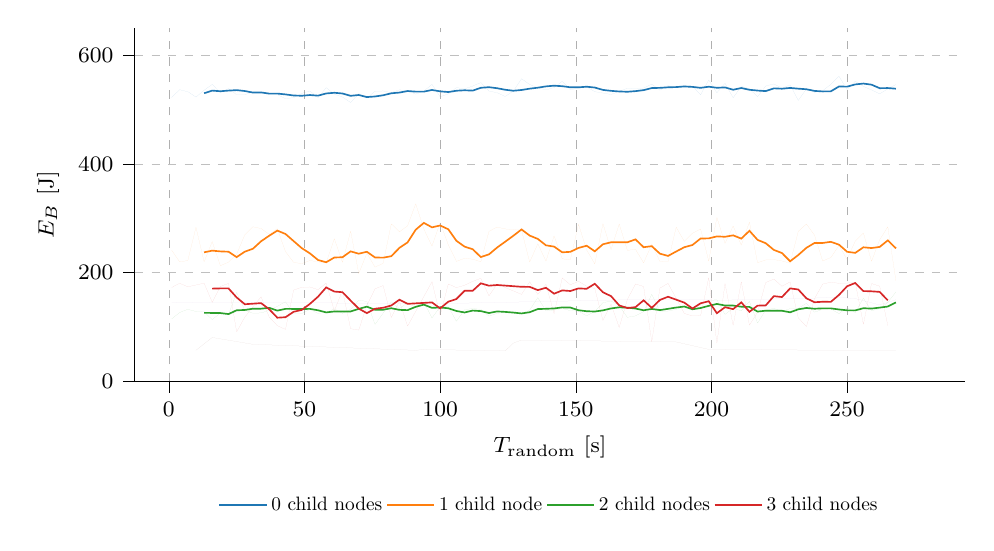
\begin{tikzpicture}

\definecolor{crimson2143940}{RGB}{214,39,40}
\definecolor{darkgray176}{RGB}{176,176,176}
\definecolor{darkorange25512714}{RGB}{255,127,14}
\definecolor{forestgreen4416044}{RGB}{44,160,44}
\definecolor{mediumpurple148103189}{RGB}{148,103,189}
\definecolor{sienna1408675}{RGB}{140,86,75}
\definecolor{steelblue31119180}{RGB}{31,119,180}

\begin{axis}[
    axis line style={black},
    axis lines* = {left},
    legend cell align={left},
    legend style={ at={(0.5,-0.3)},anchor=north, fill opacity=0.8, draw opacity=1, text opacity=1, draw=white!80.00000!black, %/tikz/column 2/.style={column sep=5pt}, /tikz/column 3/.style={column sep=5pt}
    },
    legend style={draw=none, nodes={scale=0.7, transform shape}},
    legend columns=4, 
    tick align=outside,
    tick pos=left,
    width = 1\linewidth,
    height=0.5\linewidth,
    x grid style={white!69.01960784313725!black},
    grid,
    grid style={help lines,color=gray!50, dashed},
    xtick style={color=black},
    %ylabel={energy\_per\_payload\_byte},
    ylabel={$E_{B}$ [J]},
    %xlabel={$T_a$ [\si{\minute}]},
    xlabel={$T_{\text{random}}$ [s]},
    ytick style={color=black},
    label style={font=\footnotesize},
    tick label style={font=\footnotesize, /pgf/number format/fixed},
    %ytick={0.0,0.1,0.2,0.3,0.4,5},
    %yticklabel={\pgfmathparse{\tick/60}$\pgfmathprintnumber{\pgfmathresult}$},
    %ytick={0, 180, 360, 540, 720, 900, 1080},
    %xticklabel={\pgfmathparse{(\tick/60)/30}$\pgfmathprintnumber{\pgfmathresult}$},
    clip=false,
    ymax=650,
    ymin=0
    ]
\path [fill=steelblue31119180, fill opacity=0.3]
(axis cs:1,522.298586290357)
--(axis cs:1,522.298586290357)
--(axis cs:4,536.792717243233)
--(axis cs:7,533.052956078082)
--(axis cs:10,523.085896418267)
--(axis cs:13,535.85133527414)
--(axis cs:16,546.482808698952)
--(axis cs:19,531.200382277754)
--(axis cs:22,538.811427152681)
--(axis cs:25,527.456324513056)
--(axis cs:28,527.751073428481)
--(axis cs:31,532.163260758844)
--(axis cs:34,532.404435767357)
--(axis cs:37,527.866154633009)
--(axis cs:40,527.830865092125)
--(axis cs:43,520.144756356813)
--(axis cs:46,522.19564231231)
--(axis cs:49,529.945924051583)
--(axis cs:52,534.484119444711)
--(axis cs:55,522.224491701986)
--(axis cs:58,540.432054363937)
--(axis cs:61,528.426156651509)
--(axis cs:64,523.309577216501)
--(axis cs:67,513.039582404873)
--(axis cs:70,529.70717580497)
--(axis cs:73,521.378604327958)
--(axis cs:76,533.934014602028)
--(axis cs:79,534.422108243533)
--(axis cs:82,531.321278879344)
--(axis cs:85,536.347705650401)
--(axis cs:88,535.451640723906)
--(axis cs:91,528.563602215998)
--(axis cs:94,534.255693902896)
--(axis cs:97,546.624365129629)
--(axis cs:100,523.818399955688)
--(axis cs:103,528.866316376773)
--(axis cs:106,540.607860716176)
--(axis cs:109,538.51740879201)
--(axis cs:112,543.521534160516)
--(axis cs:115,549.945248675958)
--(axis cs:118,534.351506470663)
--(axis cs:121,531.11535847359)
--(axis cs:124,524.295248443532)
--(axis cs:127,534.425265774938)
--(axis cs:130,556.938617143761)
--(axis cs:133,546.46944793416)
--(axis cs:136,540.169105078899)
--(axis cs:139,536.334663416778)
--(axis cs:142,540.753054850472)
--(axis cs:145,552.265330758728)
--(axis cs:148,536.644226457101)
--(axis cs:151,539.679450873197)
--(axis cs:154,541.927202757445)
--(axis cs:157,533.093761239827)
--(axis cs:160,530.588415260877)
--(axis cs:163,527.949787642724)
--(axis cs:166,533.935507078456)
--(axis cs:169,539.251275891505)
--(axis cs:172,538.731146302851)
--(axis cs:175,539.903613298724)
--(axis cs:178,546.978839350437)
--(axis cs:181,535.957826094379)
--(axis cs:184,544.26407810775)
--(axis cs:187,540.866319379239)
--(axis cs:190,545.412033154046)
--(axis cs:193,543.080413852828)
--(axis cs:196,527.318026509594)
--(axis cs:199,554.641590616544)
--(axis cs:202,531.030821027676)
--(axis cs:205,548.662137291081)
--(axis cs:208,521.870454004846)
--(axis cs:211,543.08468191283)
--(axis cs:214,538.483420098472)
--(axis cs:217,523.780097636848)
--(axis cs:220,543.534212575364)
--(axis cs:223,547.371712538259)
--(axis cs:226,539.689508998136)
--(axis cs:229,545.618300839945)
--(axis cs:232,517.055955161467)
--(axis cs:235,538.230142891198)
--(axis cs:238,532.01559592567)
--(axis cs:241,534.915956929302)
--(axis cs:244,546.573874701058)
--(axis cs:247,561.515309567756)
--(axis cs:250,537.005471215849)
--(axis cs:253,552.347961880818)
--(axis cs:256,542.895210961748)
--(axis cs:259,536.296935061912)
--(axis cs:262,529.054072450657)
--(axis cs:265,538.362646983262)
--(axis cs:268,546.215668486197)
--(axis cs:268,546.215668486197)
--(axis cs:268,546.215668486197)
--(axis cs:265,538.362646983262)
--(axis cs:262,529.054072450657)
--(axis cs:259,536.296935061912)
--(axis cs:256,542.895210961748)
--(axis cs:253,552.347961880818)
--(axis cs:250,537.005471215849)
--(axis cs:247,561.515309567756)
--(axis cs:244,546.573874701058)
--(axis cs:241,534.915956929302)
--(axis cs:238,532.01559592567)
--(axis cs:235,538.230142891198)
--(axis cs:232,517.055955161467)
--(axis cs:229,545.618300839945)
--(axis cs:226,539.689508998136)
--(axis cs:223,547.371712538259)
--(axis cs:220,543.534212575364)
--(axis cs:217,523.780097636848)
--(axis cs:214,538.483420098472)
--(axis cs:211,543.08468191283)
--(axis cs:208,521.870454004846)
--(axis cs:205,548.662137291081)
--(axis cs:202,531.030821027676)
--(axis cs:199,554.641590616544)
--(axis cs:196,527.318026509594)
--(axis cs:193,543.080413852828)
--(axis cs:190,545.412033154046)
--(axis cs:187,540.866319379239)
--(axis cs:184,544.26407810775)
--(axis cs:181,535.957826094379)
--(axis cs:178,546.978839350437)
--(axis cs:175,539.903613298724)
--(axis cs:172,538.731146302851)
--(axis cs:169,539.251275891505)
--(axis cs:166,533.935507078456)
--(axis cs:163,527.949787642724)
--(axis cs:160,530.588415260877)
--(axis cs:157,533.093761239827)
--(axis cs:154,541.927202757445)
--(axis cs:151,539.679450873197)
--(axis cs:148,536.644226457101)
--(axis cs:145,552.265330758728)
--(axis cs:142,540.753054850472)
--(axis cs:139,536.334663416778)
--(axis cs:136,540.169105078899)
--(axis cs:133,546.46944793416)
--(axis cs:130,556.938617143761)
--(axis cs:127,534.425265774938)
--(axis cs:124,524.295248443532)
--(axis cs:121,531.11535847359)
--(axis cs:118,534.351506470663)
--(axis cs:115,549.945248675958)
--(axis cs:112,543.521534160516)
--(axis cs:109,538.51740879201)
--(axis cs:106,540.607860716176)
--(axis cs:103,528.866316376773)
--(axis cs:100,523.818399955688)
--(axis cs:97,546.624365129629)
--(axis cs:94,534.255693902896)
--(axis cs:91,528.563602215998)
--(axis cs:88,535.451640723906)
--(axis cs:85,536.347705650401)
--(axis cs:82,531.321278879344)
--(axis cs:79,534.422108243533)
--(axis cs:76,533.934014602028)
--(axis cs:73,521.378604327958)
--(axis cs:70,529.70717580497)
--(axis cs:67,513.039582404873)
--(axis cs:64,523.309577216501)
--(axis cs:61,528.426156651509)
--(axis cs:58,540.432054363937)
--(axis cs:55,522.224491701986)
--(axis cs:52,534.484119444711)
--(axis cs:49,529.945924051583)
--(axis cs:46,522.19564231231)
--(axis cs:43,520.144756356813)
--(axis cs:40,527.830865092125)
--(axis cs:37,527.866154633009)
--(axis cs:34,532.404435767357)
--(axis cs:31,532.163260758844)
--(axis cs:28,527.751073428481)
--(axis cs:25,527.456324513056)
--(axis cs:22,538.811427152681)
--(axis cs:19,531.200382277754)
--(axis cs:16,546.482808698952)
--(axis cs:13,535.85133527414)
--(axis cs:10,523.085896418267)
--(axis cs:7,533.052956078082)
--(axis cs:4,536.792717243233)
--(axis cs:1,522.298586290357)
--cycle;

\path [fill=darkorange25512714, fill opacity=0.3]
(axis cs:1,241.351518392002)
--(axis cs:1,241.351518392002)
--(axis cs:4,219.561470715093)
--(axis cs:7,221.957592631875)
--(axis cs:10,283.40030915645)
--(axis cs:13,219.588652962359)
--(axis cs:16,256.873629711885)
--(axis cs:19,212.523876849775)
--(axis cs:22,219.066871917815)
--(axis cs:25,233.642773702942)
--(axis cs:28,269.565697440333)
--(axis cs:31,284.221743940615)
--(axis cs:34,281.069769079451)
--(axis cs:37,270.396289401544)
--(axis cs:40,280.720915813655)
--(axis cs:43,238.42566696973)
--(axis cs:46,218.649848280616)
--(axis cs:49,216.252321690078)
--(axis cs:52,222.183688850814)
--(axis cs:55,219.514905861062)
--(axis cs:58,217.890846039688)
--(axis cs:61,262.293383322768)
--(axis cs:64,218.738592823707)
--(axis cs:67,276.177609730469)
--(axis cs:70,198.137168666778)
--(axis cs:73,235.576305341004)
--(axis cs:76,209.765314208202)
--(axis cs:79,217.081496660485)
--(axis cs:82,289.683165228591)
--(axis cs:85,274.92028388917)
--(axis cs:88,285.964101662228)
--(axis cs:91,326.606845854897)
--(axis cs:94,279.969946212562)
--(axis cs:97,248.557438287241)
--(axis cs:100,292.015213188689)
--(axis cs:103,251.02843915)
--(axis cs:106,220.553954044283)
--(axis cs:109,226.166992254922)
--(axis cs:112,224.540955253209)
--(axis cs:115,219.816560881225)
--(axis cs:118,275.911362156746)
--(axis cs:121,283.584600279647)
--(axis cs:124,280.228458733295)
--(axis cs:127,279.174287355008)
--(axis cs:130,277.849295249775)
--(axis cs:133,219.208826285417)
--(axis cs:136,253.017393954114)
--(axis cs:139,221.100477854703)
--(axis cs:142,267.455395402305)
--(axis cs:145,225.201563816623)
--(axis cs:148,223.630280483846)
--(axis cs:151,288.898921383055)
--(axis cs:154,241.550213278024)
--(axis cs:157,215.964296864733)
--(axis cs:160,289.921931804243)
--(axis cs:163,242.135344433449)
--(axis cs:166,289.43156911118)
--(axis cs:169,240.829453695011)
--(axis cs:172,242.635484776106)
--(axis cs:175,217.876273432217)
--(axis cs:178,251.814443927593)
--(axis cs:181,220.36720488566)
--(axis cs:184,220.025889643993)
--(axis cs:187,283.37126148801)
--(axis cs:190,257.24425601628)
--(axis cs:193,272.329129444121)
--(axis cs:196,280.22625700109)
--(axis cs:199,221.17910551881)
--(axis cs:202,301.619158215984)
--(axis cs:205,253.6636734402)
--(axis cs:208,285.630152167582)
--(axis cs:211,250.206028193304)
--(axis cs:214,292.929837133918)
--(axis cs:217,218.043550152985)
--(axis cs:220,223.035641102179)
--(axis cs:223,223.847024063095)
--(axis cs:226,221.234378226514)
--(axis cs:229,217.188296599167)
--(axis cs:232,275.765621502206)
--(axis cs:235,289.352587596864)
--(axis cs:238,268.621164072126)
--(axis cs:241,221.173627831814)
--(axis cs:244,227.581887169914)
--(axis cs:247,249.833221631641)
--(axis cs:250,223.929959390177)
--(axis cs:253,257.966661442021)
--(axis cs:256,272.908093162079)
--(axis cs:259,220.668585053269)
--(axis cs:262,260.197470583196)
--(axis cs:265,284.139377890163)
--(axis cs:268,184.581338545127)
--(axis cs:268,184.581338545127)
--(axis cs:268,184.581338545127)
--(axis cs:265,284.139377890163)
--(axis cs:262,260.197470583196)
--(axis cs:259,220.668585053269)
--(axis cs:256,272.908093162079)
--(axis cs:253,257.966661442021)
--(axis cs:250,223.929959390177)
--(axis cs:247,249.833221631641)
--(axis cs:244,227.581887169914)
--(axis cs:241,221.173627831814)
--(axis cs:238,268.621164072126)
--(axis cs:235,289.352587596864)
--(axis cs:232,275.765621502206)
--(axis cs:229,217.188296599167)
--(axis cs:226,221.234378226514)
--(axis cs:223,223.847024063095)
--(axis cs:220,223.035641102179)
--(axis cs:217,218.043550152985)
--(axis cs:214,292.929837133918)
--(axis cs:211,250.206028193304)
--(axis cs:208,285.630152167582)
--(axis cs:205,253.6636734402)
--(axis cs:202,301.619158215984)
--(axis cs:199,221.17910551881)
--(axis cs:196,280.22625700109)
--(axis cs:193,272.329129444121)
--(axis cs:190,257.24425601628)
--(axis cs:187,283.37126148801)
--(axis cs:184,220.025889643993)
--(axis cs:181,220.36720488566)
--(axis cs:178,251.814443927593)
--(axis cs:175,217.876273432217)
--(axis cs:172,242.635484776106)
--(axis cs:169,240.829453695011)
--(axis cs:166,289.43156911118)
--(axis cs:163,242.135344433449)
--(axis cs:160,289.921931804243)
--(axis cs:157,215.964296864733)
--(axis cs:154,241.550213278024)
--(axis cs:151,288.898921383055)
--(axis cs:148,223.630280483846)
--(axis cs:145,225.201563816623)
--(axis cs:142,267.455395402305)
--(axis cs:139,221.100477854703)
--(axis cs:136,253.017393954114)
--(axis cs:133,219.208826285417)
--(axis cs:130,277.849295249775)
--(axis cs:127,279.174287355008)
--(axis cs:124,280.228458733295)
--(axis cs:121,283.584600279647)
--(axis cs:118,275.911362156746)
--(axis cs:115,219.816560881225)
--(axis cs:112,224.540955253209)
--(axis cs:109,226.166992254922)
--(axis cs:106,220.553954044283)
--(axis cs:103,251.02843915)
--(axis cs:100,292.015213188689)
--(axis cs:97,248.557438287241)
--(axis cs:94,279.969946212562)
--(axis cs:91,326.606845854897)
--(axis cs:88,285.964101662228)
--(axis cs:85,274.92028388917)
--(axis cs:82,289.683165228591)
--(axis cs:79,217.081496660485)
--(axis cs:76,209.765314208202)
--(axis cs:73,235.576305341004)
--(axis cs:70,198.137168666778)
--(axis cs:67,276.177609730469)
--(axis cs:64,218.738592823707)
--(axis cs:61,262.293383322768)
--(axis cs:58,217.890846039688)
--(axis cs:55,219.514905861062)
--(axis cs:52,222.183688850814)
--(axis cs:49,216.252321690078)
--(axis cs:46,218.649848280616)
--(axis cs:43,238.42566696973)
--(axis cs:40,280.720915813655)
--(axis cs:37,270.396289401544)
--(axis cs:34,281.069769079451)
--(axis cs:31,284.221743940615)
--(axis cs:28,269.565697440333)
--(axis cs:25,233.642773702942)
--(axis cs:22,219.066871917815)
--(axis cs:19,212.523876849775)
--(axis cs:16,256.873629711885)
--(axis cs:13,219.588652962359)
--(axis cs:10,283.40030915645)
--(axis cs:7,221.957592631875)
--(axis cs:4,219.561470715093)
--(axis cs:1,241.351518392002)
--cycle;

\path [fill=forestgreen4416044, fill opacity=0.3]
(axis cs:1,114.359619197828)
--(axis cs:1,114.359619197828)
--(axis cs:4,126.398878148345)
--(axis cs:7,132.133725659267)
--(axis cs:10,128.244170895407)
--(axis cs:13,127.456815022342)
--(axis cs:16,113.200675340636)
--(axis cs:19,125.360607212757)
--(axis cs:22,122.885276980772)
--(axis cs:25,163.160689255596)
--(axis cs:28,130.243698101603)
--(axis cs:31,125.019424945241)
--(axis cs:34,125.515991188958)
--(axis cs:37,130.504434492148)
--(axis cs:40,137.880997437129)
--(axis cs:43,146.034753008366)
--(axis cs:46,124.48472926908)
--(axis cs:49,124.472853513468)
--(axis cs:52,132.233506726001)
--(axis cs:55,124.7876313895)
--(axis cs:58,126.437644247598)
--(axis cs:61,133.13297245566)
--(axis cs:64,124.807554978475)
--(axis cs:67,132.0443421415)
--(axis cs:70,148.728349377334)
--(axis cs:73,146.816581468941)
--(axis cs:76,104.25674169761)
--(axis cs:79,125.255665839084)
--(axis cs:82,146.027942458413)
--(axis cs:85,133.50391203676)
--(axis cs:88,144.307866547679)
--(axis cs:91,134.985722726419)
--(axis cs:94,145.346857558276)
--(axis cs:97,116.110911904513)
--(axis cs:100,137.066941602157)
--(axis cs:103,137.107193593052)
--(axis cs:106,110.123233174764)
--(axis cs:109,131.410994669208)
--(axis cs:112,133.653245394646)
--(axis cs:115,132.10025740018)
--(axis cs:118,119.565718501761)
--(axis cs:121,124.667112946609)
--(axis cs:124,127.026120103265)
--(axis cs:127,127.503338044377)
--(axis cs:130,124.266015339821)
--(axis cs:133,130.709112748452)
--(axis cs:136,153.805736930154)
--(axis cs:139,129.287072174353)
--(axis cs:142,130.937776550126)
--(axis cs:145,133.729994750546)
--(axis cs:148,129.78904244658)
--(axis cs:151,128.586192530813)
--(axis cs:154,120.371110353435)
--(axis cs:157,128.173172910097)
--(axis cs:160,144.383308335895)
--(axis cs:163,147.466323619403)
--(axis cs:166,138.939039474746)
--(axis cs:169,117.422734189679)
--(axis cs:172,120.034846656027)
--(axis cs:175,128.009389780689)
--(axis cs:178,159.872562676322)
--(axis cs:181,128.419605572222)
--(axis cs:184,128.986856966697)
--(axis cs:187,132.078755956028)
--(axis cs:190,137.199834078021)
--(axis cs:193,134.541521095845)
--(axis cs:196,140.179189840655)
--(axis cs:199,148.913011711481)
--(axis cs:202,149.553879913825)
--(axis cs:205,122.810047671371)
--(axis cs:208,134.084461777253)
--(axis cs:211,129.420200862493)
--(axis cs:214,147.029909094672)
--(axis cs:217,106.81901850937)
--(axis cs:220,130.897302567988)
--(axis cs:223,133.86825051372)
--(axis cs:226,128.664692915105)
--(axis cs:229,133.308277193147)
--(axis cs:232,134.231960673893)
--(axis cs:235,143.162618370862)
--(axis cs:238,126.939307544643)
--(axis cs:241,132.268495398786)
--(axis cs:244,133.035339948267)
--(axis cs:247,124.258860075409)
--(axis cs:250,135.053896669835)
--(axis cs:253,126.26610049857)
--(axis cs:256,152.478770451818)
--(axis cs:259,129.599142030044)
--(axis cs:262,133.249212583314)
--(axis cs:265,145.049979326155)
--(axis cs:268,164.096846787297)
--(axis cs:268,164.096846787297)
--(axis cs:268,164.096846787297)
--(axis cs:265,145.049979326155)
--(axis cs:262,133.249212583314)
--(axis cs:259,129.599142030044)
--(axis cs:256,152.478770451818)
--(axis cs:253,126.26610049857)
--(axis cs:250,135.053896669835)
--(axis cs:247,124.258860075409)
--(axis cs:244,133.035339948267)
--(axis cs:241,132.268495398786)
--(axis cs:238,126.939307544643)
--(axis cs:235,143.162618370862)
--(axis cs:232,134.231960673893)
--(axis cs:229,133.308277193147)
--(axis cs:226,128.664692915105)
--(axis cs:223,133.86825051372)
--(axis cs:220,130.897302567988)
--(axis cs:217,106.81901850937)
--(axis cs:214,147.029909094672)
--(axis cs:211,129.420200862493)
--(axis cs:208,134.084461777253)
--(axis cs:205,122.810047671371)
--(axis cs:202,149.553879913825)
--(axis cs:199,148.913011711481)
--(axis cs:196,140.179189840655)
--(axis cs:193,134.541521095845)
--(axis cs:190,137.199834078021)
--(axis cs:187,132.078755956028)
--(axis cs:184,128.986856966697)
--(axis cs:181,128.419605572222)
--(axis cs:178,159.872562676322)
--(axis cs:175,128.009389780689)
--(axis cs:172,120.034846656027)
--(axis cs:169,117.422734189679)
--(axis cs:166,138.939039474746)
--(axis cs:163,147.466323619403)
--(axis cs:160,144.383308335895)
--(axis cs:157,128.173172910097)
--(axis cs:154,120.371110353435)
--(axis cs:151,128.586192530813)
--(axis cs:148,129.78904244658)
--(axis cs:145,133.729994750546)
--(axis cs:142,130.937776550126)
--(axis cs:139,129.287072174353)
--(axis cs:136,153.805736930154)
--(axis cs:133,130.709112748452)
--(axis cs:130,124.266015339821)
--(axis cs:127,127.503338044377)
--(axis cs:124,127.026120103265)
--(axis cs:121,124.667112946609)
--(axis cs:118,119.565718501761)
--(axis cs:115,132.10025740018)
--(axis cs:112,133.653245394646)
--(axis cs:109,131.410994669208)
--(axis cs:106,110.123233174764)
--(axis cs:103,137.107193593052)
--(axis cs:100,137.066941602157)
--(axis cs:97,116.110911904513)
--(axis cs:94,145.346857558276)
--(axis cs:91,134.985722726419)
--(axis cs:88,144.307866547679)
--(axis cs:85,133.50391203676)
--(axis cs:82,146.027942458413)
--(axis cs:79,125.255665839084)
--(axis cs:76,104.25674169761)
--(axis cs:73,146.816581468941)
--(axis cs:70,148.728349377334)
--(axis cs:67,132.0443421415)
--(axis cs:64,124.807554978475)
--(axis cs:61,133.13297245566)
--(axis cs:58,126.437644247598)
--(axis cs:55,124.7876313895)
--(axis cs:52,132.233506726001)
--(axis cs:49,124.472853513468)
--(axis cs:46,124.48472926908)
--(axis cs:43,146.034753008366)
--(axis cs:40,137.880997437129)
--(axis cs:37,130.504434492148)
--(axis cs:34,125.515991188958)
--(axis cs:31,125.019424945241)
--(axis cs:28,130.243698101603)
--(axis cs:25,163.160689255596)
--(axis cs:22,122.885276980772)
--(axis cs:19,125.360607212757)
--(axis cs:16,113.200675340636)
--(axis cs:13,127.456815022342)
--(axis cs:10,128.244170895407)
--(axis cs:7,132.133725659267)
--(axis cs:4,126.398878148345)
--(axis cs:1,114.359619197828)
--cycle;

\path [fill=crimson2143940, fill opacity=0.3]
(axis cs:1,172.318416406555)
--(axis cs:1,172.318416406555)
--(axis cs:4,180.172245108153)
--(axis cs:7,173.616739676988)
--(axis cs:13,180.38375026475)
--(axis cs:16,145.142870338197)
--(axis cs:19,174.256659518381)
--(axis cs:22,179.993458613465)
--(axis cs:25,90.5406167777192)
--(axis cs:28,117.735027700687)
--(axis cs:34,155.400440191169)
--(axis cs:37,117.859555478606)
--(axis cs:40,102.090604442734)
--(axis cs:43,95.1395335330382)
--(axis cs:46,167.672569822981)
--(axis cs:49,172.731496047038)
--(axis cs:52,173.330009853487)
--(axis cs:55,168.486115636669)
--(axis cs:58,180.600377235703)
--(axis cs:61,129.185197002397)
--(axis cs:64,166.998328337415)
--(axis cs:67,96.4248884288067)
--(axis cs:70,93.9352723327407)
--(axis cs:73,139.267795449188)
--(axis cs:76,169.841189028212)
--(axis cs:79,175.966127024487)
--(axis cs:82,117.143155780833)
--(axis cs:85,147.236318722531)
--(axis cs:88,101.1796272473)
--(axis cs:97,183.012975776005)
--(axis cs:100,120.813579088219)
--(axis cs:103,178.861919749255)
--(axis cs:106,172.094223594592)
--(axis cs:109,176.420036522687)
--(axis cs:112,183.664208251902)
--(axis cs:115,189.311069556752)
--(axis cs:118,157.063066461979)
--(axis cs:121,178.500399496671)
--(axis cs:130,159.761722602108)
--(axis cs:133,183.031922366504)
--(axis cs:136,159.548256468798)
--(axis cs:139,178.43671296695)
--(axis cs:142,124.109512173661)
--(axis cs:145,189.974840002922)
--(axis cs:148,177.405806163538)
--(axis cs:151,183.756891191129)
--(axis cs:154,174.75742143237)
--(axis cs:157,170.471232948891)
--(axis cs:160,111.466278730217)
--(axis cs:163,141.7107533429)
--(axis cs:166,98.74667419418)
--(axis cs:169,150.194657132961)
--(axis cs:172,178.835113771464)
--(axis cs:175,174.218281505713)
--(axis cs:178,72.4776253156835)
--(axis cs:181,171.204111106166)
--(axis cs:184,180.066338111409)
--(axis cs:190,124.649787647145)
--(axis cs:193,119.943758784077)
--(axis cs:196,120.505435189724)
--(axis cs:199,190.230704479317)
--(axis cs:202,69.8501876517088)
--(axis cs:205,179.722623325163)
--(axis cs:208,102.412809823817)
--(axis cs:211,182.959489362441)
--(axis cs:214,103.004995568886)
--(axis cs:217,126.779506865454)
--(axis cs:220,181.643543428706)
--(axis cs:223,187.855382971789)
--(axis cs:226,174.657042774233)
--(axis cs:229,182.70339101556)
--(axis cs:232,116.588840559868)
--(axis cs:235,100.312032628428)
--(axis cs:238,152.000244308707)
--(axis cs:241,178.718856254285)
--(axis cs:244,182.044979961728)
--(axis cs:247,180.119818810567)
--(axis cs:250,180.470488055137)
--(axis cs:253,182.069290456998)
--(axis cs:256,104.328937497456)
--(axis cs:259,179.705860121636)
--(axis cs:262,174.914430043836)
--(axis cs:265,102.145408961354)
--(axis cs:265,102.145408961354)
--(axis cs:265,102.145408961354)
--(axis cs:262,174.914430043836)
--(axis cs:259,179.705860121636)
--(axis cs:256,104.328937497456)
--(axis cs:253,182.069290456998)
--(axis cs:250,180.470488055137)
--(axis cs:247,180.119818810567)
--(axis cs:244,182.044979961728)
--(axis cs:241,178.718856254285)
--(axis cs:238,152.000244308707)
--(axis cs:235,100.312032628428)
--(axis cs:232,116.588840559868)
--(axis cs:229,182.70339101556)
--(axis cs:226,174.657042774233)
--(axis cs:223,187.855382971789)
--(axis cs:220,181.643543428706)
--(axis cs:217,126.779506865454)
--(axis cs:214,103.004995568886)
--(axis cs:211,182.959489362441)
--(axis cs:208,102.412809823817)
--(axis cs:205,179.722623325163)
--(axis cs:202,69.8501876517088)
--(axis cs:199,190.230704479317)
--(axis cs:196,120.505435189724)
--(axis cs:193,119.943758784077)
--(axis cs:190,124.649787647145)
--(axis cs:184,180.066338111409)
--(axis cs:181,171.204111106166)
--(axis cs:178,72.4776253156835)
--(axis cs:175,174.218281505713)
--(axis cs:172,178.835113771464)
--(axis cs:169,150.194657132961)
--(axis cs:166,98.74667419418)
--(axis cs:163,141.7107533429)
--(axis cs:160,111.466278730217)
--(axis cs:157,170.471232948891)
--(axis cs:154,174.75742143237)
--(axis cs:151,183.756891191129)
--(axis cs:148,177.405806163538)
--(axis cs:145,189.974840002922)
--(axis cs:142,124.109512173661)
--(axis cs:139,178.43671296695)
--(axis cs:136,159.548256468798)
--(axis cs:133,183.031922366504)
--(axis cs:130,159.761722602108)
--(axis cs:121,178.500399496671)
--(axis cs:118,157.063066461979)
--(axis cs:115,189.311069556752)
--(axis cs:112,183.664208251902)
--(axis cs:109,176.420036522687)
--(axis cs:106,172.094223594592)
--(axis cs:103,178.861919749255)
--(axis cs:100,120.813579088219)
--(axis cs:97,183.012975776005)
--(axis cs:88,101.1796272473)
--(axis cs:85,147.236318722531)
--(axis cs:82,117.143155780833)
--(axis cs:79,175.966127024487)
--(axis cs:76,169.841189028212)
--(axis cs:73,139.267795449188)
--(axis cs:70,93.9352723327407)
--(axis cs:67,96.4248884288067)
--(axis cs:64,166.998328337415)
--(axis cs:61,129.185197002397)
--(axis cs:58,180.600377235703)
--(axis cs:55,168.486115636669)
--(axis cs:52,173.330009853487)
--(axis cs:49,172.731496047038)
--(axis cs:46,167.672569822981)
--(axis cs:43,95.1395335330382)
--(axis cs:40,102.090604442734)
--(axis cs:37,117.859555478606)
--(axis cs:34,155.400440191169)
--(axis cs:28,117.735027700687)
--(axis cs:25,90.5406167777192)
--(axis cs:22,179.993458613465)
--(axis cs:19,174.256659518381)
--(axis cs:16,145.142870338197)
--(axis cs:13,180.38375026475)
--(axis cs:7,173.616739676988)
--(axis cs:4,180.172245108153)
--(axis cs:1,172.318416406555)
--cycle;

\path [fill=mediumpurple148103189, fill opacity=0.3]
(axis cs:1,144.13290750768)
--(axis cs:1,144.13290750768)
--(axis cs:19,145.511950132625)
--(axis cs:97,142.421531992475)
--(axis cs:178,150.621920550969)
--(axis cs:205,149.053632692567)
--(axis cs:247,154.016792068598)
--(axis cs:253,152.000100651013)
--(axis cs:262,140.337885829438)
--(axis cs:268,149.842961347582)
--(axis cs:268,149.842961347582)
--(axis cs:268,149.842961347582)
--(axis cs:262,140.337885829438)
--(axis cs:253,152.000100651013)
--(axis cs:247,154.016792068598)
--(axis cs:205,149.053632692567)
--(axis cs:178,150.621920550969)
--(axis cs:97,142.421531992475)
--(axis cs:19,145.511950132625)
--(axis cs:1,144.13290750768)
--cycle;

\path [fill=sienna1408675, fill opacity=0.3]
(axis cs:10,56.7509060700212)
--(axis cs:10,56.7509060700212)
--(axis cs:16,80.3489377491782)
--(axis cs:31,67.7513283982594)
--(axis cs:91,56.6821104049654)
--(axis cs:94,58.2381639367284)
--(axis cs:124,55.6601570957041)
--(axis cs:127,69.9414265050693)
--(axis cs:130,75.6535317718058)
--(axis cs:187,72.0667374651531)
--(axis cs:199,58.3694024456547)
--(axis cs:268,55.9735867379458)
--(axis cs:268,55.9735867379458)
--(axis cs:268,55.9735867379458)
--(axis cs:199,58.3694024456547)
--(axis cs:187,72.0667374651531)
--(axis cs:130,75.6535317718058)
--(axis cs:127,69.9414265050693)
--(axis cs:124,55.6601570957041)
--(axis cs:94,58.2381639367284)
--(axis cs:91,56.6821104049654)
--(axis cs:31,67.7513283982594)
--(axis cs:16,80.3489377491782)
--(axis cs:10,56.7509060700212)
--cycle;

\addplot [semithick, steelblue31119180]
table {%
1 nan
4 nan
7 nan
10 nan
13 530.216298260816
16 535.053142742535
19 533.934675749439
22 535.086369964359
25 535.960455583317
28 534.340403214185
31 531.476493626163
34 531.717304324084
37 529.528249820149
40 529.603157935963
43 528.081894521629
46 526.088370832323
49 525.596668489168
52 526.920261451508
55 525.798986773481
58 529.856446374906
61 531.102549242745
64 529.775279875729
67 525.486372467761
70 526.982909288358
73 523.172219281162
76 524.273790871266
79 526.496297076672
82 530.152636371567
85 531.480742340653
88 534.295349619843
91 533.221267142637
94 533.187984274509
97 536.248601524566
100 533.742740385624
103 532.425675516197
106 534.834527216233
109 535.686870194055
112 535.066304000233
115 540.291673744287
118 541.388711763065
121 539.490211314548
124 536.645779244852
127 534.826525567736
130 536.225199261297
133 538.648787553996
136 540.459536875058
139 542.867419869707
142 544.132977684814
145 543.198320407807
148 541.233276112396
151 541.135345271255
154 542.253853139389
157 540.72199441726
160 536.386611317689
163 534.647723554814
166 533.498934795866
169 532.963749422678
172 534.091226435282
175 535.954266042852
178 539.760076384394
181 540.164540187579
184 541.167100630828
187 541.594135246106
190 542.69581921717
193 541.916134117648
196 540.188174200691
199 542.26367670245
202 540.296577032138
205 540.946597859545
208 536.704605889948
211 539.857936970595
214 536.626302866981
217 535.176158188816
220 534.150573245672
223 539.250824952355
226 538.571790369416
229 539.99876651771
232 538.653938022634
235 537.593124085801
238 534.521900763283
241 533.567190349516
244 533.758305121739
247 542.650176002997
250 542.405241667927
253 546.471714858956
256 548.067565665446
259 546.012177737617
262 539.519930314197
265 539.791365467679
268 538.564906788755
};\addlegendentry{0 child nodes}
\addplot [semithick, darkorange25512714]
table {%
1 nan
4 nan
7 nan
10 nan
13 237.171908771556
16 240.276331035532
19 238.868812262469
22 238.290668119657
25 228.339161028955
28 238.33456992455
31 243.804192770296
34 257.513371216231
37 267.779254712977
40 277.19488313512
43 270.966877040999
46 257.852497908999
49 244.889008431125
52 235.246488320979
55 223.00528633046
58 218.898322144451
61 227.627029152882
64 228.124283379608
67 238.923067555539
70 234.647520116682
73 238.184611976945
76 227.678998154032
79 227.347578921388
82 230.048690021012
85 245.40531306549
88 255.482872329735
91 278.851178659074
94 291.42886856949
97 283.20372318122
100 286.622709041123
103 279.635576538678
106 258.424998176555
109 247.664407385027
112 242.86111077822
115 228.421380316728
118 233.397964918077
121 246.00409416515
124 256.816387460824
127 267.743053881184
130 279.349600754894
133 268.009093580628
136 261.895652315522
139 250.070056139803
142 247.726277749263
145 237.196731462632
148 238.081022302318
151 245.257327788106
154 249.347274872771
157 239.049055165256
160 251.99312876278
163 255.694141552701
166 255.800671098326
169 255.656519181723
172 260.990756763998
175 246.581625089593
178 248.517444988422
181 234.704572143318
184 230.543859333114
187 238.691014675495
190 246.564611192307
193 250.667548295613
196 262.639358718699
199 262.870001893662
202 266.519581239257
205 265.803464724041
208 268.463669268733
211 262.459623507176
214 276.809769830198
217 260.094648217598
220 253.969041749994
223 241.612416129096
226 235.818086135738
229 220.669778028788
232 232.214192298632
235 245.477581597569
238 254.432409599375
241 254.420259520435
244 256.498977634585
247 251.312497660472
250 238.227972019134
253 236.097071493114
256 246.443964559167
259 245.061304135838
262 247.134153926149
265 259.176037626146
268 244.498973046767
};\addlegendentry{1 child node}
\addplot [semithick, forestgreen4416044]
table {%
1 nan
4 nan
7 nan
10 nan
13 125.718641784638
16 125.486853013199
19 125.279198826082
22 123.429509090383
25 130.41281276242
28 130.970189378273
31 133.333939299194
34 133.365016094434
37 134.888847596709
40 129.832909233016
43 132.991120214369
46 132.884181079136
49 132.675553544038
52 133.021367990809
55 130.402694781283
58 126.483273029129
61 128.212921666445
64 128.279861959447
67 128.242029042547
70 133.030172640113
73 137.105960084382
76 131.330713932772
79 131.420336104894
82 134.217056168276
85 131.172168700162
88 130.670425715909
91 136.816221921671
94 140.834460265509
97 134.851054154729
100 135.563660067809
103 134.123525476883
106 129.151027566552
109 126.363854988739
112 129.872321686766
115 128.87898484637
118 125.370689828112
121 128.279465782481
124 127.402490869292
127 126.172509399238
130 124.605660987166
133 126.834339836505
136 132.662064633214
139 133.114255047431
142 133.801142748581
145 135.693938630726
148 135.509924570352
151 130.466015690484
154 128.6828233263
157 128.129902598294
160 130.260565315364
163 133.796021549929
166 135.866590938715
169 135.276915705964
172 133.64925045515
175 130.374466744109
178 132.855714555492
181 130.751827774988
184 133.064652330391
187 135.473434190392
190 137.311523049858
193 132.245314733763
196 134.597231587449
199 138.582462536406
202 142.077487327966
205 139.199530046636
208 139.108118182917
211 136.956320387285
214 136.579699863923
217 128.032727583032
220 129.650178562355
223 129.606936309649
226 129.455834720171
229 126.711508339866
232 132.194096772771
235 134.647159933346
238 133.26137133953
241 133.982131836266
244 133.92754438729
247 131.932924267593
250 130.311179927388
253 130.176538518173
256 134.21859352878
259 133.531353945135
262 135.329424446716
265 137.32864097798
268 144.894790235725
};\addlegendentry{2 child nodes}
\addplot [semithick, crimson2143940]
table {%
1 nan
4 nan
7 nan
13 nan
16 170.326804358929
19 170.714452981294
22 170.678695682356
25 154.063471102502
28 141.53372658969
34 143.585240560284
37 132.305819752329
40 116.725248918183
43 117.645032269247
46 127.632540693705
49 131.098751864879
52 142.192842739856
55 155.471944978643
58 172.564113719176
61 164.866639155059
64 163.720005613134
67 148.338981328198
70 133.428812667412
73 125.162296310109
76 133.293494715272
79 135.087054452687
82 139.230707923092
85 149.89091720105
88 142.273283560672
97 144.907640910231
100 133.877131322977
103 146.220884116662
106 151.192465091074
109 166.240546946152
112 166.370793441331
115 180.070291535038
118 175.710520877582
121 176.991756057998
130 173.660093273882
133 173.533636096803
136 167.581073479212
139 171.855802780206
142 160.977625315604
145 167.020248795767
148 165.895025555174
151 170.73675249964
154 170.000894192724
157 179.27323834777
160 163.571526093229
163 156.432515529101
166 139.430472129711
169 134.51791926983
172 136.190695434344
175 148.741095989444
178 134.894470384
181 149.385957766397
184 155.360293962087
190 144.523228737223
193 133.668324192896
196 143.273886167704
199 147.079204842334
202 125.035974750394
205 136.050541885998
208 132.544352093946
211 145.035162928489
214 127.590021146403
217 138.975884989152
220 139.360069009861
223 156.448583639455
226 154.788094321814
229 170.727773411148
232 168.689640150031
235 152.423337989976
238 145.252310257359
241 146.06467295337
244 145.932990742603
247 158.639186392743
250 174.670877478085
253 180.684686707743
256 165.806702956377
259 165.338878988359
262 164.297801235013
265 148.632785416256
};
\addlegendentry{3 child nodes}
\end{axis}

\end{tikzpicture}

    \vspace{-0.7cm}
    \caption{Simulated energy per byte ($E_B$ across the \multihop network w.r.t. the added random timer interval ($T_\text{random}$).}
    \label{fig:}
\end{figure}
\begin{figure}[p]
    \centering
    % This file was created with tikzplotlib v0.10.1.
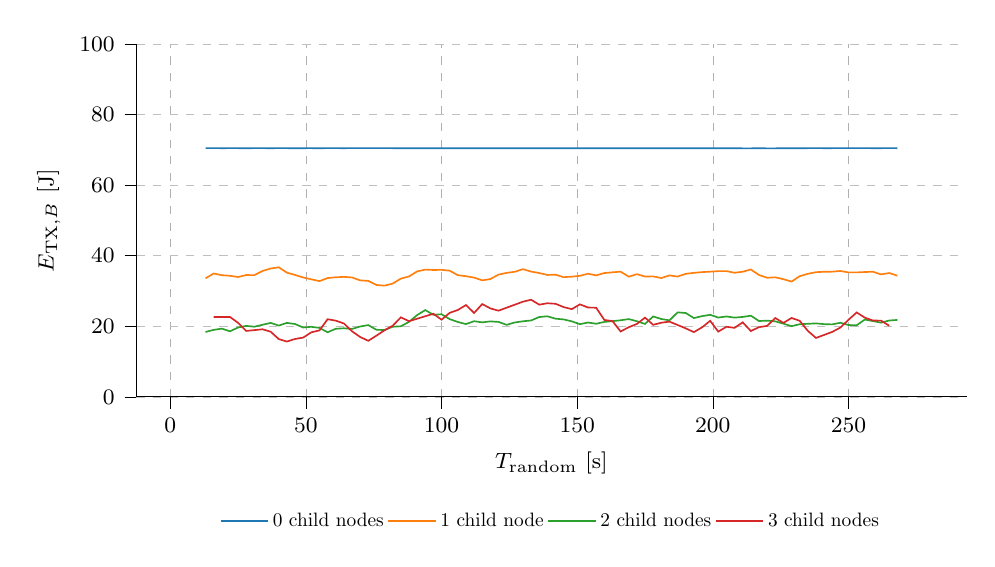
\begin{tikzpicture}

\definecolor{crimson2143940}{RGB}{214,39,40}
\definecolor{darkgray176}{RGB}{176,176,176}
\definecolor{darkorange25512714}{RGB}{255,127,14}
\definecolor{forestgreen4416044}{RGB}{44,160,44}
\definecolor{mediumpurple148103189}{RGB}{148,103,189}
\definecolor{sienna1408675}{RGB}{140,86,75}
\definecolor{steelblue31119180}{RGB}{31,119,180}

\begin{axis}[
    axis line style={black},
    axis lines* = {left},
    legend cell align={left},
    legend style={ at={(0.5,-0.3)},anchor=north, fill opacity=0.8, draw opacity=1, text opacity=1, draw=white!80.00000!black, %/tikz/column 2/.style={column sep=5pt}, /tikz/column 3/.style={column sep=5pt}
    },
    legend style={draw=none, nodes={scale=0.7, transform shape}},
    legend columns=4, 
    tick align=outside,
    tick pos=left,
    width = 1\linewidth,
    height=0.5\linewidth,
    x grid style={white!69.01960784313725!black},
    grid,
    grid style={help lines,color=gray!50, dashed},
    xtick style={color=black},
    %ylabel={energy\_per\_payload\_byte},
    ylabel={$E_{\text{TX},B}$ [J]},
    %xlabel={$T_a$ [\si{\minute}]},
    xlabel={$T_{\text{random}}$ [s]},
    ytick style={color=black},
    label style={font=\footnotesize},
    tick label style={font=\footnotesize, /pgf/number format/fixed},
    %ytick={0.0,0.1,0.2,0.3,0.4,5},
    %yticklabel={\pgfmathparse{\tick/60}$\pgfmathprintnumber{\pgfmathresult}$},
    %ytick={0, 180, 360, 540, 720, 900, 1080},
    %xticklabel={\pgfmathparse{(\tick/60)/30}$\pgfmathprintnumber{\pgfmathresult}$},
    clip=false,
    ymax=100,
    ymin=0
    ]

\addplot [semithick, steelblue31119180]
table {%
1 nan
4 nan
7 nan
10 nan
13 70.4907297257717
16 70.4906146641149
19 70.4826589723974
22 70.4866970886477
25 70.4853681265089
28 70.4774124347915
31 70.4868447511078
34 70.4867242103244
37 70.481420415846
40 70.4871159678709
43 70.4855640052824
46 70.4748358755423
49 70.4841777862708
52 70.4854434644989
55 70.4785153829615
58 70.4880230372674
61 70.4892555667799
64 70.4812998750625
67 70.491075732612
70 70.4996658495062
73 70.4927728199599
76 70.5017533822941
79 70.4986193219209
82 70.4843171579473
85 70.4743408220416
88 70.4698909638518
91 70.4555192149711
94 70.4586201266287
97 70.4601849651651
100 70.4595695727439
103 70.4655182604139
106 70.4667729803889
109 70.4612612530592
112 70.4642227209466
115 70.4643559502339
118 70.4587809389927
121 70.4617725420761
124 70.4639935060142
127 70.4609227295524
130 70.4639718634643
133 70.4651170009087
136 70.4617687066881
139 70.4650926187952
142 70.465029334884
145 70.4608350635277
148 70.462703445673
151 70.4618519894109
154 70.4618519894113
157 70.4567892765003
160 70.4635666820582
163 70.4674571358493
166 70.4641951378713
169 70.4666059535432
172 70.4748027268277
175 70.4641077458032
178 70.4625075669006
181 70.4750649030318
184 70.4631916358477
187 70.4668922379038
190 70.4777409084275
193 70.467253860255
196 70.4687288987907
199 70.4795446945551
202 70.4676473192144
205 70.4660035812561
208 70.4768884140149
211 70.4359143523456
214 70.4383881779723
217 70.4478506294847
220 70.4373800186916
223 70.4368616933217
226 70.4750950382274
229 70.4765716628264
232 70.4719054656507
235 70.4855747905103
238 70.4913607481228
241 70.4830434340547
244 70.4845501938499
247 70.4955749173598
250 70.487088846195
253 70.486929951526
256 70.4938911817784
259 70.4814152106763
262 70.483946567132
265 70.495090562575
268 70.4832967427255
};\addlegendentry{0 child nodes}
\addplot [semithick, darkorange25512714]
table {%
1 nan
4 nan
7 nan
10 nan
13 33.5915997251087
16 34.9620267102825
19 34.488217279487
22 34.3212726745534
25 33.9699752191172
28 34.5261738953743
31 34.497029428352
34 35.6863676430482
37 36.3757087461306
40 36.7253890288543
43 35.2045394382606
46 34.555607617997
49 33.8400788340962
52 33.3176823359474
55 32.8036965163968
58 33.6723365108406
61 33.899157495984
64 34.0091852106942
67 33.8470969687585
70 33.0174991708101
73 32.8622763113457
76 31.7199164849684
79 31.5215517007501
82 32.1136913141808
85 33.5077194015155
88 34.124986301024
91 35.5616923738739
94 36.0685719856303
97 35.9612683347085
100 36.0036049801882
103 35.7571760423982
106 34.4804924154537
109 34.2007910523048
112 33.7975001783692
115 33.0168872402132
118 33.3998165470226
121 34.647287181609
124 35.1417131305222
127 35.456766979559
130 36.1950432722355
133 35.5065923672426
136 35.0996880523506
139 34.5528223759093
142 34.6292053739711
145 33.9262147284689
148 34.0653911690371
151 34.3125897481195
154 34.9047868535166
157 34.4403187622799
160 35.0940541505621
163 35.3035758691805
166 35.484311577378
169 34.0655644528373
172 34.7733355538143
175 34.1186551340317
178 34.1449259328787
181 33.6720436631385
184 34.425562438144
187 34.1026434620804
190 34.8777844975735
193 35.1440525819998
196 35.3574029434949
199 35.484404888887
202 35.6303458720324
205 35.6435958350478
208 35.1779356593882
211 35.4605060541023
214 36.105887581873
217 34.5469581059585
220 33.75856710745
223 33.8871683045656
226 33.3487047969144
229 32.6798973545557
232 34.1977291262492
235 34.8810903077063
238 35.3416955611318
241 35.4534504154536
244 35.486909543522
247 35.6747779213731
250 35.2739419949788
253 35.2717796816556
256 35.3844676244071
259 35.4534040175974
262 34.710650133047
265 35.1000725153804
268 34.3317509523008
};\addlegendentry{1 child node}
\addplot [semithick, forestgreen4416044]
table {%
1 nan
4 nan
7 nan
10 nan
13 18.3913693959465
16 18.9890217179057
19 19.3389514657612
22 18.5738764786856
25 19.6607213405978
28 20.1162124481103
31 19.88457435822
34 20.4337985303804
37 20.9605883059794
40 20.2082489612457
43 20.9708136745849
46 20.6469399862492
49 19.6612086938841
52 19.8576164539744
55 19.5521261234091
58 18.3080094710087
61 19.3036349474361
64 19.4407828097338
67 19.2501687324094
70 19.9435898273123
73 20.3438334769535
76 19.0108569881989
79 18.9465494106935
82 19.8750352751689
85 20.0054974604805
88 21.2530742275882
91 23.1811815651401
94 24.5984886624102
97 23.2592375053637
100 23.4139538911504
103 22.0396612514146
106 21.220493772618
109 20.6352258749604
112 21.441264294831
115 21.1185358937238
118 21.3935618474341
121 21.2438651367868
124 20.413951614261
127 21.090160126081
130 21.4222544372462
133 21.6515531860305
136 22.6299855694809
139 22.8374068394971
142 22.1553610016412
145 21.9550566603144
148 21.4017372332075
151 20.6047570160838
154 21.0720349442279
157 20.7247227260296
160 21.2405202424608
163 21.4655054978163
166 21.7046746635702
169 22.0447503472806
172 21.4343936124077
175 20.6833343730427
178 22.790507855544
181 22.0707964901258
184 21.6871876070303
187 23.9499732855151
190 23.7708897086865
193 22.3341620061054
196 22.8780164821767
199 23.25399859099
202 22.4763141979426
205 22.7866429837847
208 22.4665935595466
211 22.6509531774593
214 23.0160166940086
217 21.4939284612003
220 21.5996170054976
223 21.4069737172021
226 20.7444185266401
229 20.0392786718144
232 20.5886595856541
235 20.7054147364757
238 20.8271133800172
241 20.6121484169083
244 20.5413657365753
247 21.0076496052635
250 20.3615643838146
253 20.2903964686629
256 21.910993746124
259 21.478127117426
262 21.027739743382
265 21.642947257895
268 21.8020530529151
};\addlegendentry{2 child nodes}
\addplot [semithick, crimson2143940]
table {%
1 nan
4 nan
7 nan
13 nan
16 22.6582523301098
19 22.6582523301098
22 22.6582523301098
25 20.9865737794772
28 18.6860844148871
34 19.155531350094
37 18.476582717561
40 16.3759954551847
43 15.6772991454283
46 16.4130278292731
49 16.7994605199702
52 18.3013967384912
55 18.8372233201222
58 22.0063597105802
61 21.6061974642163
64 20.8066811216239
67 18.5876260129681
70 16.9696017061277
73 15.890674836199
76 17.3530764761636
79 18.8912009813061
82 20.1632169076664
85 22.5477010536652
88 21.4439229718035
97 23.5547798544923
100 21.865608807669
103 23.8148034652988
106 24.6228178009907
109 26.0231714546918
112 23.7847706081516
115 26.3037958553629
118 25.0660391490352
121 24.426260403934
130 26.9756902687116
133 27.5329540092517
136 26.1306820091123
139 26.5347711351787
142 26.3832978935755
145 25.4486875536727
148 24.859967035318
151 26.2227624532161
154 25.3225389685128
157 25.2674801041636
160 21.8058273461994
163 21.4784722410387
166 18.5392591302031
169 19.7339326119243
172 20.6736317683373
175 22.4660105585676
178 20.4203447741857
181 21.0100553113691
184 21.3266327037774
190 19.4199897219579
193 18.3518702672624
196 19.6980888614089
199 21.5518363900602
202 18.4852174726344
205 19.8697050489985
208 19.5635232482652
211 21.1208603392745
214 18.6624997915164
217 19.7523647272498
220 20.1155897870542
223 22.3575682450879
226 20.9582667425858
229 22.3666361314865
232 21.5599056430221
235 18.7030231258109
238 16.7030213345357
241 17.5565329029781
244 18.417647575622
247 19.6420518269872
250 21.8526014122136
253 23.9312850865751
256 22.45933377279
259 21.6462540696517
262 21.6028314179563
265 20.1586742980787
};
\addlegendentry{3 child nodes}
\end{axis}

\end{tikzpicture}

    \vspace{-0.7cm}
    \caption{Simulated transmit energy per byte ($E_{\text{TX}, B}$ across the \multihop network w.r.t. the added random timer interval ($T_\text{random}$).}
    \label{fig:}
\end{figure}
\begin{figure}[p]
    \centering
    % This file was created with tikzplotlib v0.10.1.
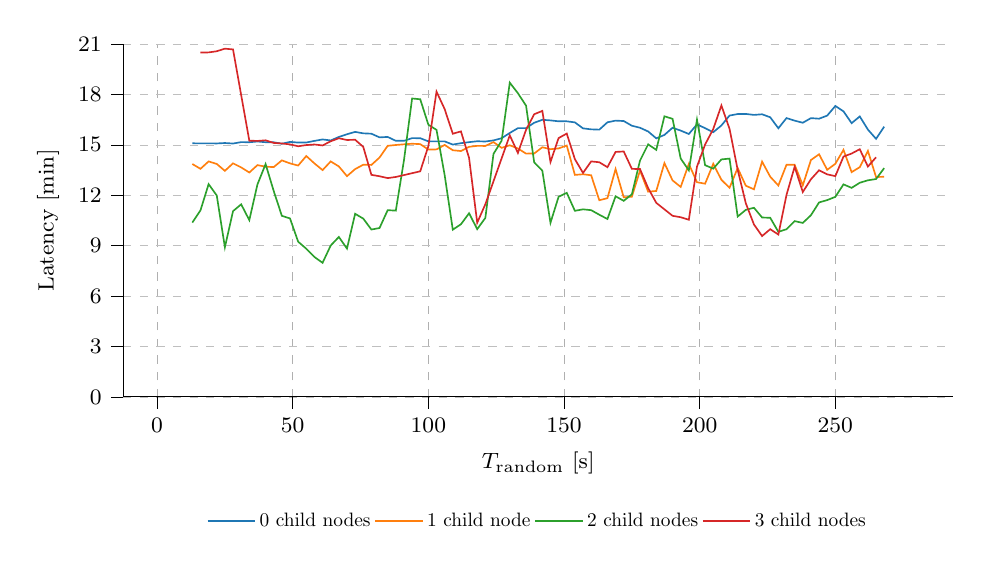
\begin{tikzpicture}

\definecolor{crimson2143940}{RGB}{214,39,40}
\definecolor{darkgray176}{RGB}{176,176,176}
\definecolor{darkorange25512714}{RGB}{255,127,14}
\definecolor{forestgreen4416044}{RGB}{44,160,44}
\definecolor{mediumpurple148103189}{RGB}{148,103,189}
\definecolor{sienna1408675}{RGB}{140,86,75}
\definecolor{steelblue31119180}{RGB}{31,119,180}

\begin{axis}[
    axis line style={black},
    axis lines* = {left},
    legend cell align={left},
    legend style={ at={(0.5,-0.3)},anchor=north, fill opacity=0.8, draw opacity=1, text opacity=1, draw=white!80.00000!black, %/tikz/column 2/.style={column sep=5pt}, /tikz/column 3/.style={column sep=5pt}
    },
    legend style={draw=none, nodes={scale=0.7, transform shape}},
    legend columns=4, 
    tick align=outside,
    tick pos=left,
    width = 1\linewidth,
    height=0.5\linewidth,
    x grid style={white!69.01960784313725!black},
    grid,
    grid style={help lines,color=gray!50, dashed},
    xtick style={color=black},
    %ylabel={energy\_per\_payload\_byte},
    ylabel={Latency [min]},
    %xlabel={$T_a$ [\si{\minute}]},
    xlabel={$T_{\text{random}}$ [s]},
    ytick style={color=black},
    label style={font=\footnotesize},
    tick label style={font=\footnotesize, /pgf/number format/fixed},
    %ytick={0.0,0.1,0.2,0.3,0.4,5},
    yticklabel={\pgfmathparse{\tick/60}$\pgfmathprintnumber{\pgfmathresult}$},
    ytick={0, 180, 360, 540, 720, 900, 1080, 1260},
    %xticklabel={\pgfmathparse{(\tick/60)/30}$\pgfmathprintnumber{\pgfmathresult}$},
    clip=false,
    ymax=1260,
    ymin=0
    ]

\addplot [semithick, steelblue31119180]
table {%
1 nan
4 nan
7 nan
10 nan
13 905.398115981427
16 905.358692693879
19 905.385706008785
22 904.952369916329
25 906.511134055859
28 904.676715009048
31 909.705964844983
34 909.285780369779
37 911.899617201287
40 909.40434737417
43 909.134102777904
46 903.985917001335
49 910.530772450135
52 908.13417983869
55 908.37558068361
58 914.093557089392
61 919.259278940054
64 915.770629824065
67 928.165980505403
70 937.93354666145
73 946.232120021294
76 941.085474951766
79 939.753551000137
82 926.668821760471
85 928.212086247218
88 914.370511516671
91 914.407949409384
94 923.850060413191
97 923.767231025464
100 912.361506068927
103 912.297632409433
106 912.321601406482
109 900.947547474469
112 905.939086940763
115 909.614146720328
118 912.803561218257
121 911.927506295827
124 915.809548271256
127 923.607497486608
130 942.438412253388
133 959.521601647803
136 959.597451478412
139 978.867718609122
142 989.425708895194
145 987.284220254223
148 984.024999820178
151 984.016990437058
154 980.221975451739
157 958.834683738051
160 955.313132447114
163 954.261557573343
166 980.483787789814
169 986.458473187894
172 984.993859509375
175 968.268791329663
178 961.033669009485
181 947.720836871525
184 923.156739528027
187 935.407382577514
190 960.991592928092
193 950.835471784861
196 938.730929298027
199 973.151976212924
202 959.497995905484
205 945.101978292027
208 969.128313994986
211 1004.54013023954
214 1009.95792498372
217 1010.35675411845
220 1006.90828602137
223 1009.09959460682
226 998.402998864954
229 959.140734478198
232 995.571388397762
235 986.358128832308
238 978.892146113522
241 995.369997877656
244 993.358326061424
247 1004.40949286074
250 1038.76816526822
253 1019.64799336378
256 977.406597283594
259 1001.42663012396
262 954.518918064545
265 921.483514296604
268 964.896250376414
};
\addlegendentry{0 child nodes}
\addplot [semithick, darkorange25512714]
table {%
1 nan
4 nan
7 nan
10 nan
13 831.59146260141
16 814.344441016823
19 840.831436976319
22 831.760569109761
25 807.101502169903
28 834.001936451316
31 819.4426226731
34 801.207984547523
37 827.651772691456
40 821.917600548823
43 820.625106740593
46 844.582365561717
49 833.776981783565
52 826.034545770837
55 860.126797755903
58 833.728716599414
61 809.822877080782
64 840.759609965603
67 822.927770828668
70 788.161918952122
73 813.341954329275
76 828.985985283573
79 828.268211340724
82 854.669380633828
85 896.552824828316
88 899.457060489643
91 901.807922928815
94 903.907720019723
97 902.544940524496
100 883.266054503998
103 883.683681064701
106 899.632486951388
109 880.710060908677
112 877.826265678569
115 892.936519130621
118 896.38801118289
121 896.03594059595
124 909.736423410796
127 889.296380661428
130 898.436687123959
133 887.000532438277
136 868.713390958712
139 869.078937918145
142 891.348016038285
145 884.488560231375
148 887.202752814494
151 897.627532780059
154 792.631559838347
157 794.936381423235
160 791.338996742132
163 702.129477716478
166 709.629677683346
169 813.564864431598
172 712.577897716789
175 714.768250920156
178 808.350049212276
181 732.746329885985
184 735.303342031243
187 834.858454212613
190 773.008867058746
193 749.684012300819
196 831.770940512491
199 766.570998787342
202 761.286532919828
205 832.305647019383
208 775.054625070992
211 746.800465888384
214 817.144015096427
217 754.003802879741
220 741.190405355276
223 840.164288259882
226 786.058782408955
229 754.882005212022
232 828.950045139068
235 829.032372118691
238 755.279834104703
241 845.742971509438
244 866.31283620947
247 810.676498882115
250 832.366430134715
253 882.062339316448
256 802.539386075857
259 820.217838102277
262 878.421783957307
265 784.991256071152
268 786.075647708668
};
\addlegendentry{1 child node}
\addplot [semithick, forestgreen4416044]
table {%
1 nan
4 nan
7 nan
10 nan
13 622.239439854943
16 666.055342880077
19 759.632271079225
22 719.194357768239
25 534.332675426791
28 663.217403868156
31 687.60999201446
34 631.159682741244
37 758.710642519773
40 831.437126929541
43 734.996274842102
46 646.482475716534
49 637.183064794745
52 554.130848741401
55 529.028364883269
58 499.535154380035
61 478.74050566862
64 540.479975721519
67 571.040090067892
70 529.600555983751
73 653.819006690545
76 636.547131919964
79 597.557654064703
82 602.942532158742
85 666.740384534391
88 665.011508860806
91 844.714611874796
94 1065.53067348797
97 1062.75550519283
100 971.77165403849
103 953.511052054076
106 791.979618911784
109 597.039157901769
112 616.319236353518
115 655.66054882504
118 598.930503281937
121 639.117290956743
124 867.655106173349
127 914.813152953495
130 1122.04859710235
133 1084.33887994792
136 1040.0041418825
139 837.489742635169
142 807.74672934039
145 621.552320502117
148 714.614040323174
151 728.665263064505
154 664.400066562533
157 669.695088745294
160 666.709865696024
163 650.462893965266
166 635.165654301053
169 716.269578449724
172 700.111021134174
175 723.269225306755
178 843.648856583584
181 901.815298885433
184 882.001116365788
187 1001.92879278684
190 992.901892234361
193 851.035080189199
196 808.772233531687
199 989.981302302848
202 827.338980947343
205 814.966349890039
208 848.011078280147
211 850.855028793853
214 643.945138259459
217 667.831755193463
220 675.350586427489
223 640.516806991361
226 639.439428548635
229 589.297357974014
232 598.677698709893
235 627.599356505613
238 621.156417328468
241 648.594213207093
244 694.329268246379
247 702.709438822644
250 714.382648195248
253 758.823580801041
256 746.36119982666
259 764.586656772972
262 773.36012110773
265 777.892431862077
268 816.912829080432
};
\addlegendentry{2 child nodes}
\addplot [semithick, crimson2143940]
table {%
1 nan
4 nan
7 nan
13 nan
16 1229.69905132016
19 1230.05937388689
22 1234.24389146665
25 1243.40052710774
28 1240.73408234679
34 914.874435842737
37 913.971354046991
40 916.152808837832
43 906.83917383945
46 904.921536135303
49 901.668073265224
52 894.926899006299
55 899.175529911815
58 901.234572976719
61 897.848550940511
64 912.721124484964
67 923.537042831814
70 917.304420483334
73 918.156184756883
76 892.66995303507
79 792.828878189185
82 787.873101499793
85 781.226480848412
88 785.270040600946
97 805.516264446012
100 895.596319028689
103 1090.00731671765
106 1027.73210973686
109 939.646246663373
112 948.045066960083
115 853.460102544096
118 621.827916523523
121 687.872246987456
130 933.791568534829
133 871.117372939545
136 953.602969204869
139 1009.26865479761
142 1021.16413030474
145 838.775417744106
148 924.153527275969
151 940.256975393825
154 848.818930260178
157 799.815084139069
160 840.817673541126
163 837.813420818675
166 820.163817658936
169 874.666071406492
172 876.313545281195
175 814.229689166474
178 813.565698228719
181 745.69161009284
184 692.780087184596
190 646.574188874646
193 641.47861017854
196 632.529556236246
199 822.154340404859
202 901.179151115089
205 956.710451987337
208 1040.517449292
211 957.204116984813
214 811.06858918909
217 691.352009148857
220 615.686978948486
223 574.256774186748
226 598.813954365184
229 579.582018875698
232 721.347913857713
235 821.856294627196
238 731.517217840086
241 777.055873460808
244 809.211134703013
247 794.538513596044
250 788.272183352712
253 858.102689262965
256 868.933878122865
259 884.415736062882
262 822.415669878844
265 855.514774984773
};
\addlegendentry{3 child nodes}
\end{axis}

\end{tikzpicture}

    \vspace{-0.7cm}
    \caption{Simulated latency of sensor readings across the \multihop network w.r.t. the added random timer interval ($T_\text{random}$).}
    \label{fig:}
\end{figure}




%%%%%%%%%%%%%%%%%%%%%%%%%%%%%%%%%%%%%%%%%%%%%%%%PAYLOAD SIZE%%%%%%%%%%%%%%%%%%%%%%%%%%%%%%%%%%%%%%%%%%%%%%
\FloatBarrier
\begin{figure}[p]
    \centering
    % This file was created with tikzplotlib v0.10.1.
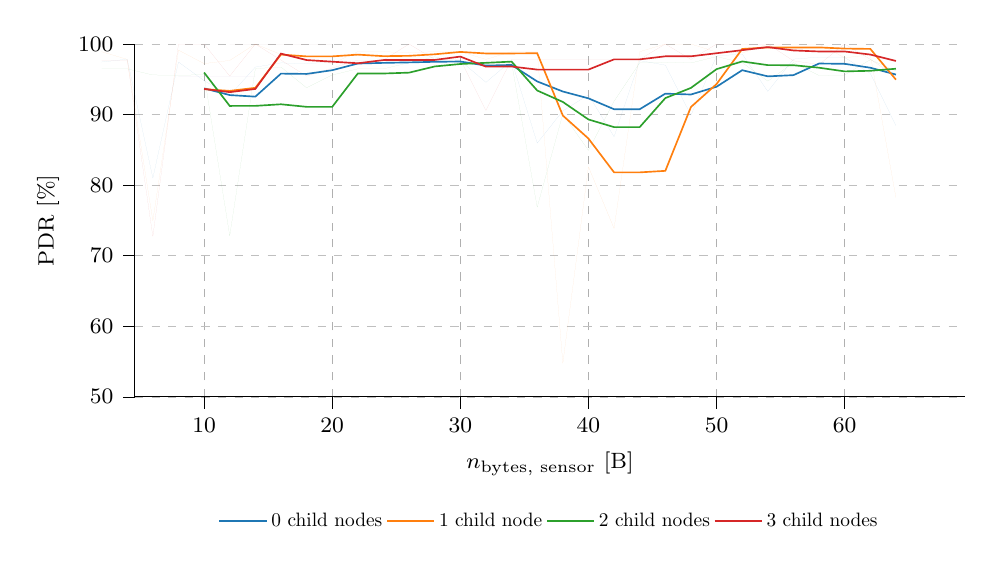
\begin{tikzpicture}

\definecolor{crimson2143940}{RGB}{214,39,40}
\definecolor{darkgray176}{RGB}{176,176,176}
\definecolor{darkorange25512714}{RGB}{255,127,14}
\definecolor{forestgreen4416044}{RGB}{44,160,44}
\definecolor{mediumpurple148103189}{RGB}{148,103,189}
\definecolor{sienna1408675}{RGB}{140,86,75}
\definecolor{steelblue31119180}{RGB}{31,119,180}

\begin{axis}[
    axis line style={black},
    axis lines* = {left},
    legend cell align={left},
    legend style={ at={(0.5,-0.3)},anchor=north, fill opacity=0.8, draw opacity=1, text opacity=1, draw=white!80.00000!black, %/tikz/column 2/.style={column sep=5pt}, /tikz/column 3/.style={column sep=5pt}
    },
    legend style={draw=none, nodes={scale=0.7, transform shape}},
    legend columns=4, 
    tick align=outside,
    tick pos=left,
    width = 1\linewidth,
    height=0.5\linewidth,
    x grid style={white!69.01960784313725!black},
    grid,
    grid style={help lines,color=gray!50, dashed},
    xtick style={color=black},
    %ylabel={energy\_per\_payload\_byte},
    ylabel={PDR [\%]},
    %xlabel={$T_a$ [\si{\minute}]},
    xlabel={$n_{\text{bytes, sensor}}$ [B]},
    ytick style={color=black},
    label style={font=\footnotesize},
    tick label style={font=\footnotesize, /pgf/number format/fixed},
    ytick={0.5,0.6,0.7,0.8,0.9,1},
    yticklabel={\pgfmathparse{100*\tick}$\pgfmathprintnumber{\pgfmathresult}$},
    %xtick={0, 180, 360, 540, 720, 900, 1080, 1260, 1440, 1620, 1800},
    %xticklabel={\pgfmathparse{(\tick/60)/30}$\pgfmathprintnumber{\pgfmathresult}$},
    clip=false,
    ymax=1,
    ymin=0.5
    ]
\path [fill=steelblue31119180, fill opacity=0.3]
(axis cs:2,0.974496517974779)
--(axis cs:2,0.974496517974779)
--(axis cs:4,0.9785431959345)
--(axis cs:6,0.810097425004257)
--(axis cs:8,0.974496517974779)
--(axis cs:10,0.94802371541502)
--(axis cs:12,0.927146963708228)
--(axis cs:14,0.967391304347826)
--(axis cs:16,0.973221343873518)
--(axis cs:18,0.972332015810277)
--(axis cs:20,0.974393446443136)
--(axis cs:22,0.974496517974779)
--(axis cs:24,0.972040726699112)
--(axis cs:26,0.976492614936551)
--(axis cs:28,0.97656691134952)
--(axis cs:30,0.976472802559759)
--(axis cs:32,0.945712672420747)
--(axis cs:34,0.97656691134952)
--(axis cs:36,0.859603129789465)
--(axis cs:38,0.905259336936356)
--(axis cs:40,0.927966443494394)
--(axis cs:42,0.868610685380872)
--(axis cs:44,0.97656691134952)
--(axis cs:46,0.970064442114132)
--(axis cs:48,0.899128210393032)
--(axis cs:50,0.983060417843027)
--(axis cs:52,0.985853962970668)
--(axis cs:54,0.932846656449141)
--(axis cs:56,0.978628341982379)
--(axis cs:58,0.981477679106138)
--(axis cs:60,0.980841431642347)
--(axis cs:62,0.958295689817429)
--(axis cs:64,0.884486166007905)
--(axis cs:64,0.884486166007905)
--(axis cs:64,0.884486166007905)
--(axis cs:62,0.958295689817429)
--(axis cs:60,0.980841431642347)
--(axis cs:58,0.981477679106138)
--(axis cs:56,0.978628341982379)
--(axis cs:54,0.932846656449141)
--(axis cs:52,0.985853962970668)
--(axis cs:50,0.983060417843027)
--(axis cs:48,0.899128210393032)
--(axis cs:46,0.970064442114132)
--(axis cs:44,0.97656691134952)
--(axis cs:42,0.868610685380872)
--(axis cs:40,0.927966443494394)
--(axis cs:38,0.905259336936356)
--(axis cs:36,0.859603129789465)
--(axis cs:34,0.97656691134952)
--(axis cs:32,0.945712672420747)
--(axis cs:30,0.976472802559759)
--(axis cs:28,0.97656691134952)
--(axis cs:26,0.976492614936551)
--(axis cs:24,0.972040726699112)
--(axis cs:22,0.974496517974779)
--(axis cs:20,0.974393446443136)
--(axis cs:18,0.972332015810277)
--(axis cs:16,0.973221343873518)
--(axis cs:14,0.967391304347826)
--(axis cs:12,0.927146963708228)
--(axis cs:10,0.94802371541502)
--(axis cs:8,0.974496517974779)
--(axis cs:6,0.810097425004257)
--(axis cs:4,0.9785431959345)
--(axis cs:2,0.974496517974779)
--cycle;

\path [fill=darkorange25512714, fill opacity=0.3]
(axis cs:2,0.989130434782609)
--(axis cs:2,0.989130434782609)
--(axis cs:4,0.978260869565217)
--(axis cs:6,0.749458874458874)
--(axis cs:8,0.991304347826087)
--(axis cs:10,0.972294372294372)
--(axis cs:12,0.976731601731602)
--(axis cs:14,1)
--(axis cs:16,0.985177865612648)
--(axis cs:18,0.978260869565217)
--(axis cs:20,0.972294372294372)
--(axis cs:22,0.989130434782609)
--(axis cs:24,0.989130434782609)
--(axis cs:26,0.987577639751553)
--(axis cs:28,0.989130434782609)
--(axis cs:30,0.989130434782609)
--(axis cs:32,0.978260869565217)
--(axis cs:34,0.989130434782609)
--(axis cs:36,0.989130434782609)
--(axis cs:38,0.547619047619048)
--(axis cs:40,0.826086956521739)
--(axis cs:42,0.738612836438923)
--(axis cs:44,0.989130434782609)
--(axis cs:46,1)
--(axis cs:48,1)
--(axis cs:50,0.988636363636364)
--(axis cs:52,0.98729531338227)
--(axis cs:54,1)
--(axis cs:56,1)
--(axis cs:58,1)
--(axis cs:60,0.980492592293835)
--(axis cs:62,0.984848484848485)
--(axis cs:64,0.782213438735178)
--(axis cs:64,0.782213438735178)
--(axis cs:64,0.782213438735178)
--(axis cs:62,0.984848484848485)
--(axis cs:60,0.980492592293835)
--(axis cs:58,1)
--(axis cs:56,1)
--(axis cs:54,1)
--(axis cs:52,0.98729531338227)
--(axis cs:50,0.988636363636364)
--(axis cs:48,1)
--(axis cs:46,1)
--(axis cs:44,0.989130434782609)
--(axis cs:42,0.738612836438923)
--(axis cs:40,0.826086956521739)
--(axis cs:38,0.547619047619048)
--(axis cs:36,0.989130434782609)
--(axis cs:34,0.989130434782609)
--(axis cs:32,0.978260869565217)
--(axis cs:30,0.989130434782609)
--(axis cs:28,0.989130434782609)
--(axis cs:26,0.987577639751553)
--(axis cs:24,0.989130434782609)
--(axis cs:22,0.989130434782609)
--(axis cs:20,0.972294372294372)
--(axis cs:18,0.978260869565217)
--(axis cs:16,0.985177865612648)
--(axis cs:14,1)
--(axis cs:12,0.976731601731602)
--(axis cs:10,0.972294372294372)
--(axis cs:8,0.991304347826087)
--(axis cs:6,0.749458874458874)
--(axis cs:4,0.978260869565217)
--(axis cs:2,0.989130434782609)
--cycle;

\path [fill=forestgreen4416044, fill opacity=0.3]
(axis cs:2,0.964822134387352)
--(axis cs:2,0.964822134387352)
--(axis cs:4,0.964822134387352)
--(axis cs:6,0.956126482213439)
--(axis cs:8,0.95602766798419)
--(axis cs:10,0.956192358366271)
--(axis cs:12,0.728260869565217)
--(axis cs:14,0.965217391304348)
--(axis cs:16,0.967391304347826)
--(axis cs:18,0.937944664031621)
--(axis cs:20,0.956126482213439)
--(axis cs:22,0.964822134387352)
--(axis cs:24,0.964822134387352)
--(axis cs:26,0.973517786561265)
--(axis cs:28,0.981818181818182)
--(axis cs:30,0.973517786561265)
--(axis cs:32,0.973084886128364)
--(axis cs:34,0.973517786561265)
--(axis cs:36,0.76875588179936)
--(axis cs:38,0.900790513833992)
--(axis cs:40,0.849275362318841)
--(axis cs:42,0.91897233201581)
--(axis cs:44,0.973517786561265)
--(axis cs:46,0.974281412169611)
--(axis cs:48,0.973122529644269)
--(axis cs:50,0.982213438735178)
--(axis cs:52,0.973517786561265)
--(axis cs:54,0.947430830039526)
--(axis cs:56,0.973517786561265)
--(axis cs:58,0.955533596837945)
--(axis cs:60,0.956126482213439)
--(axis cs:62,0.977766798418972)
--(axis cs:64,0.962058472928038)
--(axis cs:64,0.962058472928038)
--(axis cs:64,0.962058472928038)
--(axis cs:62,0.977766798418972)
--(axis cs:60,0.956126482213439)
--(axis cs:58,0.955533596837945)
--(axis cs:56,0.973517786561265)
--(axis cs:54,0.947430830039526)
--(axis cs:52,0.973517786561265)
--(axis cs:50,0.982213438735178)
--(axis cs:48,0.973122529644269)
--(axis cs:46,0.974281412169611)
--(axis cs:44,0.973517786561265)
--(axis cs:42,0.91897233201581)
--(axis cs:40,0.849275362318841)
--(axis cs:38,0.900790513833992)
--(axis cs:36,0.76875588179936)
--(axis cs:34,0.973517786561265)
--(axis cs:32,0.973084886128364)
--(axis cs:30,0.973517786561265)
--(axis cs:28,0.981818181818182)
--(axis cs:26,0.973517786561265)
--(axis cs:24,0.964822134387352)
--(axis cs:22,0.964822134387352)
--(axis cs:20,0.956126482213439)
--(axis cs:18,0.937944664031621)
--(axis cs:16,0.967391304347826)
--(axis cs:14,0.965217391304348)
--(axis cs:12,0.728260869565217)
--(axis cs:10,0.956192358366271)
--(axis cs:8,0.95602766798419)
--(axis cs:6,0.956126482213439)
--(axis cs:4,0.964822134387352)
--(axis cs:2,0.964822134387352)
--cycle;

\path [fill=crimson2143940, fill opacity=0.3]
(axis cs:2,0.977272727272727)
--(axis cs:2,0.977272727272727)
--(axis cs:4,0.977272727272727)
--(axis cs:6,0.727272727272727)
--(axis cs:8,1)
--(axis cs:10,1)
--(axis cs:12,0.954545454545455)
--(axis cs:14,1)
--(axis cs:16,0.977272727272727)
--(axis cs:18,0.954545454545455)
--(axis cs:22,0.977272727272727)
--(axis cs:24,0.977272727272727)
--(axis cs:26,1)
--(axis cs:28,0.978260869565217)
--(axis cs:30,0.978260869565217)
--(axis cs:32,0.905844155844156)
--(axis cs:34,0.978260869565217)
--(axis cs:36,0.978260869565217)
--(axis cs:38,0.978260869565217)
--(axis cs:40,0.978260869565217)
--(axis cs:42,0.978260869565217)
--(axis cs:44,0.978260869565217)
--(axis cs:46,1)
--(axis cs:48,0.978260869565217)
--(axis cs:50,1)
--(axis cs:52,1)
--(axis cs:54,1)
--(axis cs:56,0.976190476190476)
--(axis cs:58,0.971014492753623)
--(axis cs:60,1)
--(axis cs:62,0.978260869565217)
--(axis cs:64,0.954545454545455)
--(axis cs:64,0.954545454545455)
--(axis cs:64,0.954545454545455)
--(axis cs:62,0.978260869565217)
--(axis cs:60,1)
--(axis cs:58,0.971014492753623)
--(axis cs:56,0.976190476190476)
--(axis cs:54,1)
--(axis cs:52,1)
--(axis cs:50,1)
--(axis cs:48,0.978260869565217)
--(axis cs:46,1)
--(axis cs:44,0.978260869565217)
--(axis cs:42,0.978260869565217)
--(axis cs:40,0.978260869565217)
--(axis cs:38,0.978260869565217)
--(axis cs:36,0.978260869565217)
--(axis cs:34,0.978260869565217)
--(axis cs:32,0.905844155844156)
--(axis cs:30,0.978260869565217)
--(axis cs:28,0.978260869565217)
--(axis cs:26,1)
--(axis cs:24,0.977272727272727)
--(axis cs:22,0.977272727272727)
--(axis cs:18,0.954545454545455)
--(axis cs:16,0.977272727272727)
--(axis cs:14,1)
--(axis cs:12,0.954545454545455)
--(axis cs:10,1)
--(axis cs:8,1)
--(axis cs:6,0.727272727272727)
--(axis cs:4,0.977272727272727)
--(axis cs:2,0.977272727272727)
--cycle;

\path [fill=mediumpurple148103189, fill opacity=0.3]
(axis cs:8,0.954545454545455)
--(axis cs:8,0.954545454545455)
--(axis cs:14,0.954545454545455)
--(axis cs:14,0.954545454545455)
--(axis cs:14,0.954545454545455)
--(axis cs:8,0.954545454545455)
--cycle;

\path [fill=sienna1408675, fill opacity=0.3]
(axis cs:12,1)
--(axis cs:12,1)
--(axis cs:20,1)
--(axis cs:20,1)
--(axis cs:20,1)
--(axis cs:12,1)
--cycle;

\addplot [semithick, steelblue31119180]
table {%
2 nan
4 nan
6 nan
8 nan
10 0.937131474460667
12 0.927661563607357
14 0.925431185290022
16 0.958055969063874
18 0.957623068630974
20 0.962897014836597
22 0.972366925689907
24 0.973296810160164
26 0.973951064372771
28 0.974798043480619
30 0.975213914703944
32 0.969457145593138
34 0.970362382523219
36 0.946984485493802
38 0.932722970611169
40 0.923021698798096
42 0.907601301390121
44 0.907601301390121
46 0.929693563855055
48 0.92846733854639
50 0.939486133416117
52 0.962934788934076
54 0.954190737954
56 0.955903517927649
58 0.97237341167027
60 0.971929614430134
62 0.966417959799487
64 0.95674586171124
};
\addlegendentry{0 child nodes}
\addplot [semithick, darkorange25512714]
table {%
2 nan
4 nan
6 nan
8 nan
10 0.936089779785432
12 0.933610013175231
14 0.937957839262187
16 0.985101637492942
18 0.982492941840768
20 0.982492941840768
22 0.984972708450969
24 0.982798795407491
26 0.983278750235272
28 0.98545266327875
30 0.988819875776398
32 0.986645962732919
34 0.986645962732919
36 0.986956521739131
38 0.898654244306418
40 0.866045548654244
42 0.818115942028986
44 0.818115942028986
46 0.820289855072464
48 0.910766045548654
50 0.943275926971579
52 0.993012422360249
54 0.995186335403727
56 0.995186335403727
58 0.995186335403727
60 0.993557581135221
62 0.993068215428464
64 0.949510903175499
};
\addlegendentry{1 child node}
\addplot [semithick, forestgreen4416044]
table {%
2 nan
4 nan
6 nan
8 nan
10 0.959598155467721
12 0.912285902503294
14 0.912364953886693
16 0.91461791831357
18 0.911001317523057
20 0.91098814229249
22 0.958300395256917
24 0.958221343873518
26 0.959446640316206
28 0.968221343873518
30 0.971699604743083
32 0.973352155091285
34 0.975091285526068
36 0.934138904573687
38 0.917933370976849
40 0.893084886128364
42 0.882262375305854
44 0.882262375305854
46 0.923367481379904
48 0.937833884541959
50 0.964421499825227
52 0.975330590734317
54 0.97011319942997
56 0.9699604743083
58 0.966442687747036
60 0.961225296442688
62 0.962075098814229
64 0.965000627391932
};
\addlegendentry{2 child nodes}
\addplot [semithick, crimson2143940]
table {%
2 nan
4 nan
6 nan
8 nan
10 0.936363636363636
12 0.931818181818182
14 0.936363636363636
16 0.986363636363636
18 0.977272727272727
22 0.972727272727273
24 0.977272727272727
26 0.977272727272727
28 0.977470355731225
30 0.982213438735178
32 0.967927724449464
34 0.968125352907962
36 0.963777526821005
38 0.963777526821005
40 0.963777526821005
42 0.978260869565217
44 0.978260869565217
46 0.982608695652174
48 0.982608695652174
50 0.986956521739131
52 0.991304347826087
54 0.995652173913043
56 0.990890269151139
58 0.98944099378882
60 0.98944099378882
62 0.985093167701863
64 0.976002258610954
};
\addlegendentry{3 child nodes}
\end{axis}

\end{tikzpicture}

    \vspace{-0.7cm}
    \caption{Simulated packet delivery ratio (PDR) across the \multihop network w.r.t. the data size of one sensor value ($n_\text{bytes, sensor}$).}
    \label{fig:}
\end{figure}
\begin{figure}[p]
    \centering
    % This file was created with tikzplotlib v0.10.1.
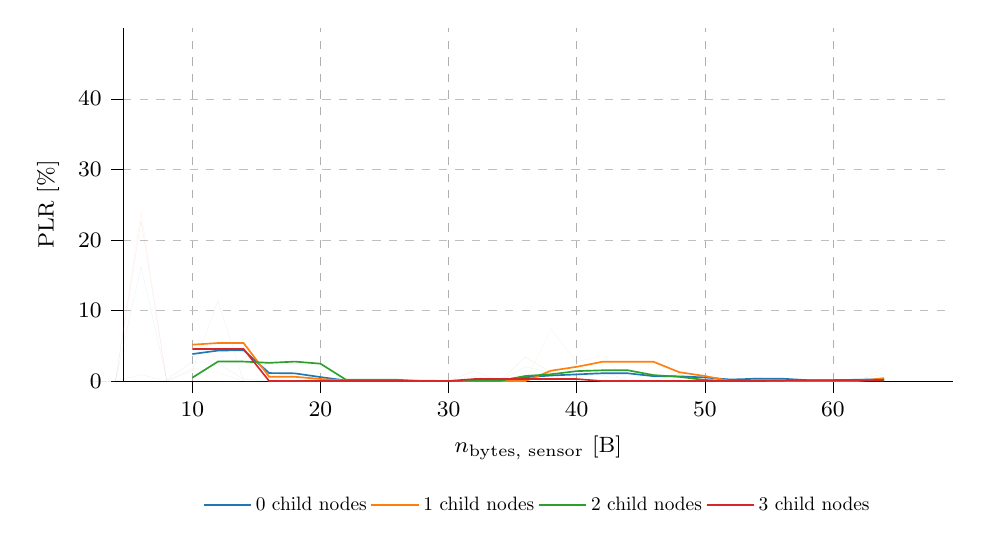
\begin{tikzpicture}

\definecolor{crimson2143940}{RGB}{214,39,40}
\definecolor{darkgray176}{RGB}{176,176,176}
\definecolor{darkorange25512714}{RGB}{255,127,14}
\definecolor{forestgreen4416044}{RGB}{44,160,44}
\definecolor{mediumpurple148103189}{RGB}{148,103,189}
\definecolor{sienna1408675}{RGB}{140,86,75}
\definecolor{steelblue31119180}{RGB}{31,119,180}

\begin{axis}[
    axis line style={black},
    axis lines* = {left},
    legend cell align={left},
    legend style={ at={(0.5,-0.3)},anchor=north, fill opacity=0.8, draw opacity=1, text opacity=1, draw=white!80.00000!black, %/tikz/column 2/.style={column sep=5pt}, /tikz/column 3/.style={column sep=5pt}
    },
    legend style={draw=none, nodes={scale=0.7, transform shape}},
    legend columns=4, 
    tick align=outside,
    tick pos=left,
    width = 1\linewidth,
    height=0.5\linewidth,
    x grid style={white!69.01960784313725!black},
    grid,
    grid style={help lines,color=gray!50, dashed},
    xtick style={color=black},
    %ylabel={energy\_per\_payload\_byte},
    ylabel={PLR [\%]},
    %xlabel={$T_a$ [\si{\minute}]},
    xlabel={$n_{\text{bytes, sensor}}$ [B]},
    ytick style={color=black},
    label style={font=\footnotesize},
    tick label style={font=\footnotesize, /pgf/number format/fixed},
    ytick={0.0,0.1,0.2,0.3,0.4,5},
    yticklabel={\pgfmathparse{100*\tick}$\pgfmathprintnumber{\pgfmathresult}$},
    %xtick={0, 180, 360, 540, 720, 900, 1080, 1260, 1440, 1620, 1800},
    %xticklabel={\pgfmathparse{(\tick/60)/30}$\pgfmathprintnumber{\pgfmathresult}$},
    clip=false,
    ymax=0.5,
    ymin=0
    ]
\path [fill=steelblue31119180, fill opacity=0.3]
(axis cs:2,0)
--(axis cs:2,0)
--(axis cs:4,0)
--(axis cs:6,0.162234590806019)
--(axis cs:8,0.0020703933747412)
--(axis cs:10,0.0272727272727273)
--(axis cs:12,0.0242544017247575)
--(axis cs:14,0.003099173553719)
--(axis cs:16,0)
--(axis cs:18,0)
--(axis cs:20,0.000755857898715038)
--(axis cs:22,0)
--(axis cs:24,0.000566893424036281)
--(axis cs:26,0)
--(axis cs:28,0)
--(axis cs:30,0)
--(axis cs:32,0.00658492646070284)
--(axis cs:34,0.000414078674948238)
--(axis cs:36,0.0201840947182562)
--(axis cs:38,0.0122139764996908)
--(axis cs:40,0.00773932761510401)
--(axis cs:42,0.0147744397966226)
--(axis cs:44,0)
--(axis cs:46,0)
--(axis cs:48,0.0108348091302637)
--(axis cs:50,0)
--(axis cs:52,0)
--(axis cs:54,0.00556885028934717)
--(axis cs:56,0.000481996341209586)
--(axis cs:58,0.000481000481000473)
--(axis cs:60,0.000250626566416037)
--(axis cs:62,0.00261904761904762)
--(axis cs:64,0.0099901185770751)
--(axis cs:64,0.0099901185770751)
--(axis cs:64,0.0099901185770751)
--(axis cs:62,0.00261904761904762)
--(axis cs:60,0.000250626566416037)
--(axis cs:58,0.000481000481000473)
--(axis cs:56,0.000481996341209586)
--(axis cs:54,0.00556885028934717)
--(axis cs:52,0)
--(axis cs:50,0)
--(axis cs:48,0.0108348091302637)
--(axis cs:46,0)
--(axis cs:44,0)
--(axis cs:42,0.0147744397966226)
--(axis cs:40,0.00773932761510401)
--(axis cs:38,0.0122139764996908)
--(axis cs:36,0.0201840947182562)
--(axis cs:34,0.000414078674948238)
--(axis cs:32,0.00658492646070284)
--(axis cs:30,0)
--(axis cs:28,0)
--(axis cs:26,0)
--(axis cs:24,0.000566893424036281)
--(axis cs:22,0)
--(axis cs:20,0.000755857898715038)
--(axis cs:18,0)
--(axis cs:16,0)
--(axis cs:14,0.003099173553719)
--(axis cs:12,0.0242544017247575)
--(axis cs:10,0.0272727272727273)
--(axis cs:8,0.0020703933747412)
--(axis cs:6,0.162234590806019)
--(axis cs:4,0)
--(axis cs:2,0)
--cycle;

\path [fill=darkorange25512714, fill opacity=0.3]
(axis cs:2,0)
--(axis cs:2,0)
--(axis cs:4,0)
--(axis cs:6,0.239177489177489)
--(axis cs:8,0)
--(axis cs:10,0.0186147186147186)
--(axis cs:12,0.0116341991341991)
--(axis cs:14,0)
--(axis cs:16,0)
--(axis cs:18,0)
--(axis cs:20,0.00317460317460316)
--(axis cs:22,0)
--(axis cs:24,0)
--(axis cs:26,0)
--(axis cs:28,0)
--(axis cs:30,0)
--(axis cs:32,0)
--(axis cs:34,0)
--(axis cs:36,0)
--(axis cs:38,0.0735852311939268)
--(axis cs:40,0.0271739130434782)
--(axis cs:42,0.0357882283348122)
--(axis cs:44,0)
--(axis cs:46,0)
--(axis cs:48,0)
--(axis cs:50,0)
--(axis cs:52,0)
--(axis cs:54,0)
--(axis cs:56,0)
--(axis cs:58,0)
--(axis cs:60,0.000680272108843529)
--(axis cs:62,0)
--(axis cs:64,0.02)
--(axis cs:64,0.02)
--(axis cs:64,0.02)
--(axis cs:62,0)
--(axis cs:60,0.000680272108843529)
--(axis cs:58,0)
--(axis cs:56,0)
--(axis cs:54,0)
--(axis cs:52,0)
--(axis cs:50,0)
--(axis cs:48,0)
--(axis cs:46,0)
--(axis cs:44,0)
--(axis cs:42,0.0357882283348122)
--(axis cs:40,0.0271739130434782)
--(axis cs:38,0.0735852311939268)
--(axis cs:36,0)
--(axis cs:34,0)
--(axis cs:32,0)
--(axis cs:30,0)
--(axis cs:28,0)
--(axis cs:26,0)
--(axis cs:24,0)
--(axis cs:22,0)
--(axis cs:20,0.00317460317460316)
--(axis cs:18,0)
--(axis cs:16,0)
--(axis cs:14,0)
--(axis cs:12,0.0116341991341991)
--(axis cs:10,0.0186147186147186)
--(axis cs:8,0)
--(axis cs:6,0.239177489177489)
--(axis cs:4,0)
--(axis cs:2,0)
--cycle;

\path [fill=forestgreen4416044, fill opacity=0.3]
(axis cs:2,0)
--(axis cs:2,0)
--(axis cs:4,0)
--(axis cs:6,0.00909090909090908)
--(axis cs:8,0)
--(axis cs:10,0.0148221343873518)
--(axis cs:12,0.114130434782609)
--(axis cs:14,0)
--(axis cs:16,0)
--(axis cs:18,0.00895915678524372)
--(axis cs:20,0)
--(axis cs:22,0)
--(axis cs:24,0)
--(axis cs:26,0)
--(axis cs:28,0)
--(axis cs:30,0)
--(axis cs:32,0.0019047619047619)
--(axis cs:34,0)
--(axis cs:36,0.0341269841269841)
--(axis cs:38,0.0121212121212121)
--(axis cs:40,0.0222222222222222)
--(axis cs:42,0.00779220779220778)
--(axis cs:44,0)
--(axis cs:46,0)
--(axis cs:48,0)
--(axis cs:50,0)
--(axis cs:52,0)
--(axis cs:54,0.00289855072463768)
--(axis cs:56,0)
--(axis cs:58,0.00120772946859903)
--(axis cs:60,0)
--(axis cs:62,0)
--(axis cs:64,0.00231193926846098)
--(axis cs:64,0.00231193926846098)
--(axis cs:64,0.00231193926846098)
--(axis cs:62,0)
--(axis cs:60,0)
--(axis cs:58,0.00120772946859903)
--(axis cs:56,0)
--(axis cs:54,0.00289855072463768)
--(axis cs:52,0)
--(axis cs:50,0)
--(axis cs:48,0)
--(axis cs:46,0)
--(axis cs:44,0)
--(axis cs:42,0.00779220779220778)
--(axis cs:40,0.0222222222222222)
--(axis cs:38,0.0121212121212121)
--(axis cs:36,0.0341269841269841)
--(axis cs:34,0)
--(axis cs:32,0.0019047619047619)
--(axis cs:30,0)
--(axis cs:28,0)
--(axis cs:26,0)
--(axis cs:24,0)
--(axis cs:22,0)
--(axis cs:20,0)
--(axis cs:18,0.00895915678524372)
--(axis cs:16,0)
--(axis cs:14,0)
--(axis cs:12,0.114130434782609)
--(axis cs:10,0.0148221343873518)
--(axis cs:8,0)
--(axis cs:6,0.00909090909090908)
--(axis cs:4,0)
--(axis cs:2,0)
--cycle;

\path [fill=crimson2143940, fill opacity=0.3]
(axis cs:2,0)
--(axis cs:2,0)
--(axis cs:4,0)
--(axis cs:6,0.227272727272727)
--(axis cs:8,0)
--(axis cs:10,0)
--(axis cs:12,0)
--(axis cs:14,0)
--(axis cs:16,0)
--(axis cs:18,0)
--(axis cs:22,0)
--(axis cs:24,0)
--(axis cs:26,0)
--(axis cs:28,0)
--(axis cs:30,0)
--(axis cs:32,0.0142857142857143)
--(axis cs:34,0)
--(axis cs:36,0)
--(axis cs:38,0)
--(axis cs:40,0)
--(axis cs:42,0)
--(axis cs:44,0)
--(axis cs:46,0)
--(axis cs:48,0)
--(axis cs:50,0)
--(axis cs:52,0)
--(axis cs:54,0)
--(axis cs:56,0.0026455026455026)
--(axis cs:58,0.00161030595813203)
--(axis cs:60,0)
--(axis cs:62,0)
--(axis cs:64,0.0045454545454545)
--(axis cs:64,0.0045454545454545)
--(axis cs:64,0.0045454545454545)
--(axis cs:62,0)
--(axis cs:60,0)
--(axis cs:58,0.00161030595813203)
--(axis cs:56,0.0026455026455026)
--(axis cs:54,0)
--(axis cs:52,0)
--(axis cs:50,0)
--(axis cs:48,0)
--(axis cs:46,0)
--(axis cs:44,0)
--(axis cs:42,0)
--(axis cs:40,0)
--(axis cs:38,0)
--(axis cs:36,0)
--(axis cs:34,0)
--(axis cs:32,0.0142857142857143)
--(axis cs:30,0)
--(axis cs:28,0)
--(axis cs:26,0)
--(axis cs:24,0)
--(axis cs:22,0)
--(axis cs:18,0)
--(axis cs:16,0)
--(axis cs:14,0)
--(axis cs:12,0)
--(axis cs:10,0)
--(axis cs:8,0)
--(axis cs:6,0.227272727272727)
--(axis cs:4,0)
--(axis cs:2,0)
--cycle;

\path [fill=mediumpurple148103189, fill opacity=0.3]
(axis cs:8,0)
--(axis cs:8,0)
--(axis cs:14,0)
--(axis cs:14,0)
--(axis cs:14,0)
--(axis cs:8,0)
--cycle;

\path [fill=sienna1408675, fill opacity=0.3]
(axis cs:12,0)
--(axis cs:12,0)
--(axis cs:20,0)
--(axis cs:20,0)
--(axis cs:20,0)
--(axis cs:12,0)
--cycle;

\addplot [semithick, steelblue31119180]
table {%
2 nan
4 nan
6 nan
8 nan
10 0.0383155422906976
12 0.0431664226356491
14 0.0437862573463929
16 0.011339339185189
18 0.0109252605102407
20 0.0056218866354383
22 0.000771006290486809
24 0.000264550264550264
26 0.000264550264550264
28 0.000264550264550264
30 0.000113378684807256
32 0.00143036397694782
34 0.00139980102713022
36 0.00543661997078145
38 0.00787941527071961
40 0.00942728079374041
42 0.0110651834609244
44 0.0109823677259347
46 0.00694554878228347
48 0.00666971530839805
50 0.00512184978537725
52 0.00216696182605273
54 0.00328073188392217
56 0.00337713115216409
58 0.00130636942231145
60 0.00135649473559465
62 0.00188030425940418
64 0.00276455791694976
};
\addlegendentry{0 child nodes}
\addplot [semithick, darkorange25512714]
table {%
2 nan
4 nan
6 nan
8 nan
10 0.0515584415584416
12 0.0538852813852814
14 0.0538852813852814
16 0.00604978354978355
18 0.00604978354978355
20 0.00296176046176046
22 0.000634920634920632
24 0.000634920634920632
26 0.000634920634920632
28 0.000634920634920632
30 0
32 0
34 0
36 0
38 0.0147170462387854
40 0.020151828847481
42 0.0273094745144434
44 0.0273094745144434
46 0.0273094745144434
48 0.0125924282756581
50 0.00715764566696244
52 0
54 0
56 0
58 0
60 0.000136054421768706
62 0.000136054421768706
64 0.00413605442176871
};
\addlegendentry{1 child nodes}
\addplot [semithick, forestgreen4416044]
table {%
2 nan
4 nan
6 nan
8 nan
10 0.00478260869565217
12 0.0276086956521739
14 0.0276086956521739
16 0.0257905138339921
18 0.0275823451910408
20 0.0246179183135705
22 0.00179183135704874
24 0.00179183135704874
26 0.00179183135704874
28 0
30 0
32 0.00038095238095238
34 0.00038095238095238
36 0.0072063492063492
38 0.00963059163059163
40 0.0140750360750361
42 0.0152525252525252
44 0.0152525252525252
46 0.00842712842712842
48 0.006002886002886
50 0.00155844155844156
52 0
54 0.000579710144927536
56 0.000579710144927536
58 0.000821256038647341
60 0.000821256038647341
62 0.000821256038647341
64 0.000703933747412002
};
\addlegendentry{2 child nodes}
\addplot [semithick, crimson2143940]
table {%
2 nan
4 nan
6 nan
8 nan
10 0.0454545454545454
12 0.0454545454545454
14 0.0454545454545454
16 0
18 0
22 0
24 0
26 0
28 0
30 0
32 0.00285714285714285
34 0.00285714285714285
36 0.00285714285714285
38 0.00285714285714285
40 0.00285714285714285
42 0
44 0
46 0
48 0
50 0
52 0
54 0
56 0.00052910052910052
58 0.000851161720726927
60 0.000851161720726927
62 0.000851161720726927
64 0.00176025262981783
};
\addlegendentry{3 child nodes}
\end{axis}

\end{tikzpicture}

    \vspace{-0.7cm}
    \caption{Simulated packet loss ratio (PLR) by collisions across the \multihop network w.r.t. the data size of one sensor value ($n_\text{bytes, sensor}$).}
    \label{fig:}
\end{figure}
\begin{figure}[p]
    \centering
    % This file was created with tikzplotlib v0.10.1.
\begin{tikzpicture}

\definecolor{crimson2143940}{RGB}{214,39,40}
\definecolor{darkgray176}{RGB}{176,176,176}
\definecolor{darkorange25512714}{RGB}{255,127,14}
\definecolor{forestgreen4416044}{RGB}{44,160,44}
\definecolor{mediumpurple148103189}{RGB}{148,103,189}
\definecolor{sienna1408675}{RGB}{140,86,75}
\definecolor{steelblue31119180}{RGB}{31,119,180}

\begin{axis}[
tick align=outside,
tick pos=left,
unbounded coords=jump,
x grid style={darkgray176},
xlabel={MEASURE_PAYLOAD_SIZE_BYTE},
xmin=-1.1, xmax=67.1,
xtick style={color=black},
y grid style={darkgray176},
ymin=-0.04921875, ymax=1.03359375,
ytick style={color=black}
]
\path [fill=steelblue31119180, fill opacity=0.3]
(axis cs:2,0)
--(axis cs:2,0)
--(axis cs:4,0)
--(axis cs:6,0)
--(axis cs:8,0)
--(axis cs:10,0)
--(axis cs:12,0)
--(axis cs:14,0)
--(axis cs:16,0)
--(axis cs:18,0)
--(axis cs:20,0)
--(axis cs:22,0)
--(axis cs:24,0)
--(axis cs:26,0)
--(axis cs:28,0)
--(axis cs:30,0)
--(axis cs:32,0)
--(axis cs:34,0)
--(axis cs:36,0)
--(axis cs:38,0)
--(axis cs:40,0)
--(axis cs:42,0)
--(axis cs:44,0)
--(axis cs:46,0)
--(axis cs:48,0)
--(axis cs:50,0)
--(axis cs:52,0)
--(axis cs:54,0)
--(axis cs:56,0)
--(axis cs:58,0)
--(axis cs:60,0)
--(axis cs:62,0)
--(axis cs:64,0)
--(axis cs:64,0)
--(axis cs:64,0)
--(axis cs:62,0)
--(axis cs:60,0)
--(axis cs:58,0)
--(axis cs:56,0)
--(axis cs:54,0)
--(axis cs:52,0)
--(axis cs:50,0)
--(axis cs:48,0)
--(axis cs:46,0)
--(axis cs:44,0)
--(axis cs:42,0)
--(axis cs:40,0)
--(axis cs:38,0)
--(axis cs:36,0)
--(axis cs:34,0)
--(axis cs:32,0)
--(axis cs:30,0)
--(axis cs:28,0)
--(axis cs:26,0)
--(axis cs:24,0)
--(axis cs:22,0)
--(axis cs:20,0)
--(axis cs:18,0)
--(axis cs:16,0)
--(axis cs:14,0)
--(axis cs:12,0)
--(axis cs:10,0)
--(axis cs:8,0)
--(axis cs:6,0)
--(axis cs:4,0)
--(axis cs:2,0)
--cycle;

\path [fill=darkorange25512714, fill opacity=0.3]
(axis cs:2,0.915158102766798)
--(axis cs:2,0.915158102766798)
--(axis cs:4,0.904397233201581)
--(axis cs:6,0.924324769433465)
--(axis cs:8,0.914735177865613)
--(axis cs:10,0.913735177865613)
--(axis cs:12,0.913908102766798)
--(axis cs:14,0.926877470355731)
--(axis cs:16,0.921974088713219)
--(axis cs:18,0.904397233201581)
--(axis cs:20,0.922760210803689)
--(axis cs:22,0.915158102766798)
--(axis cs:24,0.915158102766798)
--(axis cs:26,0.90416149068323)
--(axis cs:28,0.896141304347826)
--(axis cs:30,0.896141304347826)
--(axis cs:32,0.875760869565217)
--(axis cs:34,0.896141304347826)
--(axis cs:36,0.896141304347826)
--(axis cs:38,0.896141304347826)
--(axis cs:40,0.895647233201581)
--(axis cs:42,0.904891304347826)
--(axis cs:44,0.896141304347826)
--(axis cs:46,0.902177283451298)
--(axis cs:48,0.831020066889632)
--(axis cs:50,0.905344202898551)
--(axis cs:52,0.860093058273038)
--(axis cs:54,0.895271739130435)
--(axis cs:56,0.818115750528541)
--(axis cs:58,0.831020066889632)
--(axis cs:60,0.857204137285027)
--(axis cs:62,0.837077167019027)
--(axis cs:64,0.915151515151515)
--(axis cs:64,0.915151515151515)
--(axis cs:64,0.915151515151515)
--(axis cs:62,0.837077167019027)
--(axis cs:60,0.857204137285027)
--(axis cs:58,0.831020066889632)
--(axis cs:56,0.818115750528541)
--(axis cs:54,0.895271739130435)
--(axis cs:52,0.860093058273038)
--(axis cs:50,0.905344202898551)
--(axis cs:48,0.831020066889632)
--(axis cs:46,0.902177283451298)
--(axis cs:44,0.896141304347826)
--(axis cs:42,0.904891304347826)
--(axis cs:40,0.895647233201581)
--(axis cs:38,0.896141304347826)
--(axis cs:36,0.896141304347826)
--(axis cs:34,0.896141304347826)
--(axis cs:32,0.875760869565217)
--(axis cs:30,0.896141304347826)
--(axis cs:28,0.896141304347826)
--(axis cs:26,0.90416149068323)
--(axis cs:24,0.915158102766798)
--(axis cs:22,0.915158102766798)
--(axis cs:20,0.922760210803689)
--(axis cs:18,0.904397233201581)
--(axis cs:16,0.921974088713219)
--(axis cs:14,0.926877470355731)
--(axis cs:12,0.913908102766798)
--(axis cs:10,0.913735177865613)
--(axis cs:8,0.914735177865613)
--(axis cs:6,0.924324769433465)
--(axis cs:4,0.904397233201581)
--(axis cs:2,0.915158102766798)
--cycle;

\path [fill=forestgreen4416044, fill opacity=0.3]
(axis cs:2,0.913015503875969)
--(axis cs:2,0.913015503875969)
--(axis cs:4,0.908971014492754)
--(axis cs:6,0.903974789915966)
--(axis cs:8,0.910340909090909)
--(axis cs:10,0.912201213818861)
--(axis cs:12,0.909968487394958)
--(axis cs:14,0.916546218487395)
--(axis cs:16,0.919810606060606)
--(axis cs:18,0.833415458937198)
--(axis cs:20,0.823780126849894)
--(axis cs:22,0.920793281653747)
--(axis cs:24,0.919383838383838)
--(axis cs:26,0.929759261706533)
--(axis cs:28,0.948525419829768)
--(axis cs:30,0.947600644122383)
--(axis cs:32,0.837613594135333)
--(axis cs:34,0.90382960035134)
--(axis cs:36,0.878453430627344)
--(axis cs:38,0.940337536859276)
--(axis cs:40,0.930351966873706)
--(axis cs:42,0.94947895100069)
--(axis cs:44,0.946095492354074)
--(axis cs:46,0.866597611452783)
--(axis cs:48,0.857979797979798)
--(axis cs:50,0.781916842847075)
--(axis cs:52,0.855811965811966)
--(axis cs:54,0.942331982438365)
--(axis cs:56,0.778700854700855)
--(axis cs:58,0.843806485911749)
--(axis cs:60,0.778242521367521)
--(axis cs:62,0.729428904428904)
--(axis cs:64,0.881378774482223)
--(axis cs:64,0.881378774482223)
--(axis cs:64,0.881378774482223)
--(axis cs:62,0.729428904428904)
--(axis cs:60,0.778242521367521)
--(axis cs:58,0.843806485911749)
--(axis cs:56,0.778700854700855)
--(axis cs:54,0.942331982438365)
--(axis cs:52,0.855811965811966)
--(axis cs:50,0.781916842847075)
--(axis cs:48,0.857979797979798)
--(axis cs:46,0.866597611452783)
--(axis cs:44,0.946095492354074)
--(axis cs:42,0.94947895100069)
--(axis cs:40,0.930351966873706)
--(axis cs:38,0.940337536859276)
--(axis cs:36,0.878453430627344)
--(axis cs:34,0.90382960035134)
--(axis cs:32,0.837613594135333)
--(axis cs:30,0.947600644122383)
--(axis cs:28,0.948525419829768)
--(axis cs:26,0.929759261706533)
--(axis cs:24,0.919383838383838)
--(axis cs:22,0.920793281653747)
--(axis cs:20,0.823780126849894)
--(axis cs:18,0.833415458937198)
--(axis cs:16,0.919810606060606)
--(axis cs:14,0.916546218487395)
--(axis cs:12,0.909968487394958)
--(axis cs:10,0.912201213818861)
--(axis cs:8,0.910340909090909)
--(axis cs:6,0.903974789915966)
--(axis cs:4,0.908971014492754)
--(axis cs:2,0.913015503875969)
--cycle;

\path [fill=crimson2143940, fill opacity=0.3]
(axis cs:2,0.914855072463768)
--(axis cs:2,0.914855072463768)
--(axis cs:4,0.914855072463768)
--(axis cs:6,0.928921568627451)
--(axis cs:8,0.954545454545455)
--(axis cs:10,0.941176470588235)
--(axis cs:12,0.916666666666667)
--(axis cs:14,0.91304347826087)
--(axis cs:16,0.916666666666667)
--(axis cs:18,0.914855072463768)
--(axis cs:22,0.914855072463768)
--(axis cs:24,0.914855072463768)
--(axis cs:26,0.976744186046512)
--(axis cs:28,0.948701298701299)
--(axis cs:30,0.948701298701299)
--(axis cs:32,0.95672268907563)
--(axis cs:34,0.948701298701299)
--(axis cs:36,0.948701298701299)
--(axis cs:38,0.959800664451827)
--(axis cs:40,0.959800664451827)
--(axis cs:42,0.959800664451827)
--(axis cs:44,0.959800664451827)
--(axis cs:46,0.984375)
--(axis cs:48,0.733080808080808)
--(axis cs:50,0.966149870801034)
--(axis cs:52,0.956521739130435)
--(axis cs:54,0.955436720142602)
--(axis cs:56,0.955882352941176)
--(axis cs:58,0.948068924539513)
--(axis cs:60,0.956521739130435)
--(axis cs:62,0.956984273820537)
--(axis cs:64,0.955555555555556)
--(axis cs:64,0.955555555555556)
--(axis cs:64,0.955555555555556)
--(axis cs:62,0.956984273820537)
--(axis cs:60,0.956521739130435)
--(axis cs:58,0.948068924539513)
--(axis cs:56,0.955882352941176)
--(axis cs:54,0.955436720142602)
--(axis cs:52,0.956521739130435)
--(axis cs:50,0.966149870801034)
--(axis cs:48,0.733080808080808)
--(axis cs:46,0.984375)
--(axis cs:44,0.959800664451827)
--(axis cs:42,0.959800664451827)
--(axis cs:40,0.959800664451827)
--(axis cs:38,0.959800664451827)
--(axis cs:36,0.948701298701299)
--(axis cs:34,0.948701298701299)
--(axis cs:32,0.95672268907563)
--(axis cs:30,0.948701298701299)
--(axis cs:28,0.948701298701299)
--(axis cs:26,0.976744186046512)
--(axis cs:24,0.914855072463768)
--(axis cs:22,0.914855072463768)
--(axis cs:18,0.914855072463768)
--(axis cs:16,0.916666666666667)
--(axis cs:14,0.91304347826087)
--(axis cs:12,0.916666666666667)
--(axis cs:10,0.941176470588235)
--(axis cs:8,0.954545454545455)
--(axis cs:6,0.928921568627451)
--(axis cs:4,0.914855072463768)
--(axis cs:2,0.914855072463768)
--cycle;

\path [fill=mediumpurple148103189, fill opacity=0.3]
(axis cs:8,0.941176470588235)
--(axis cs:8,0.941176470588235)
--(axis cs:14,0.942857142857143)
--(axis cs:14,0.942857142857143)
--(axis cs:14,0.942857142857143)
--(axis cs:8,0.941176470588235)
--cycle;

\path [fill=sienna1408675, fill opacity=0.3]
(axis cs:12,0.955555555555556)
--(axis cs:12,0.955555555555556)
--(axis cs:20,0.956521739130435)
--(axis cs:20,0.956521739130435)
--(axis cs:20,0.956521739130435)
--(axis cs:12,0.955555555555556)
--cycle;

\addplot [semithick, steelblue31119180]
table {%
2 nan
4 nan
6 nan
8 nan
10 0
12 0
14 0
16 0
18 0
20 0
22 0
24 0
26 0
28 0
30 0
32 0
34 0
36 0
38 0
40 0
42 0
44 0
46 0
48 0
50 0
52 0
54 0
56 0
58 0
60 0
62 0
64 0
};
\addplot [semithick, darkorange25512714]
table {%
2 nan
4 nan
6 nan
8 nan
10 0.914470092226614
12 0.914220092226614
14 0.918716139657444
16 0.918246003513395
18 0.916178414580589
20 0.917983421168204
22 0.918233421168204
24 0.915889547650417
26 0.912327028044419
28 0.910675842273668
30 0.905352060982496
32 0.89747261434218
34 0.893669254658385
36 0.892065217391304
38 0.892065217391304
40 0.891966403162055
42 0.897792490118577
44 0.897792490118577
46 0.898999685939271
48 0.885975438447632
50 0.887914832387027
52 0.878955183172069
54 0.878781270128591
56 0.86196896354404
58 0.86196896354404
60 0.852340950421335
62 0.847737772170533
64 0.851713727374749
};
\addplot [semithick, forestgreen4416044]
table {%
2 nan
4 nan
6 nan
8 nan
10 0.909700686238892
12 0.90909128294269
14 0.910606323741618
16 0.913773486970546
18 0.898388396939804
20 0.88070417954601
22 0.882869138397768
24 0.883436662377057
26 0.885426393506242
28 0.908448385684756
30 0.933212489139254
32 0.916576551635571
34 0.913465704029071
36 0.903204537813233
38 0.901566961219135
40 0.8981172257694
42 0.920490297142471
44 0.928943475543018
46 0.926572311708106
48 0.91010076393221
50 0.880413739126884
52 0.861680342089139
54 0.860927640105998
56 0.843348288755612
58 0.840513626342002
60 0.839778762046091
62 0.814502149769479
64 0.80231150817825
};
\addplot [semithick, crimson2143940]
table {%
2 nan
4 nan
6 nan
8 nan
10 0.930870727737735
12 0.931233046578315
14 0.930870727737735
16 0.928419747345579
18 0.920481670929241
22 0.915217391304348
24 0.914855072463768
26 0.927595214020897
28 0.934002140427823
30 0.940771385675329
32 0.949144908997701
34 0.955914154245208
36 0.950305576776165
38 0.952525449926271
40 0.954745323076376
42 0.955360918151616
44 0.957580791301721
46 0.964715531561462
48 0.919371560287258
50 0.920641401557099
52 0.919985616492821
54 0.919112827630976
56 0.913414298219211
58 0.956411921510952
60 0.954486295176832
62 0.954578802114853
64 0.954602569197443
};
\addplot [semithick, mediumpurple148103189]
table {%
8 nan
14 nan
};
\addplot [semithick, sienna1408675]
table {%
12 nan
20 nan
};
\end{axis}

\end{tikzpicture}

    \vspace{-0.7cm}
    \caption{Simulated Simulated aggregation ratio $\alpha_\text{aggregation}$ across the \multihop network w.r.t. the data size of one sensor value ($n_\text{bytes, sensor}$).}
    \label{fig:}
\end{figure}
\begin{figure}[p]
    \centering
    % This file was created with tikzplotlib v0.10.1.
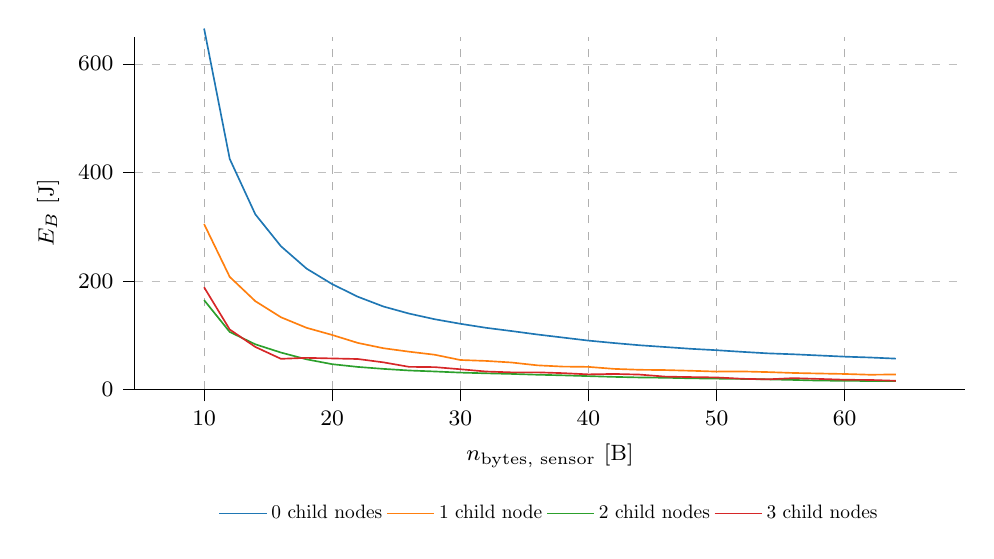
\begin{tikzpicture}

\definecolor{crimson2143940}{RGB}{214,39,40}
\definecolor{darkgray176}{RGB}{176,176,176}
\definecolor{darkorange25512714}{RGB}{255,127,14}
\definecolor{forestgreen4416044}{RGB}{44,160,44}
\definecolor{mediumpurple148103189}{RGB}{148,103,189}
\definecolor{sienna1408675}{RGB}{140,86,75}
\definecolor{steelblue31119180}{RGB}{31,119,180}

\begin{axis}[
    axis line style={black},
    axis lines* = {left},
    legend cell align={left},
    legend style={ at={(0.5,-0.3)},anchor=north, fill opacity=0.8, draw opacity=1, text opacity=1, draw=white!80.00000!black, %/tikz/column 2/.style={column sep=5pt}, /tikz/column 3/.style={column sep=5pt}
    },
    legend style={draw=none, nodes={scale=0.7, transform shape}},
    legend columns=4, 
    tick align=outside,
    tick pos=left,
    width = 1\linewidth,
    height=0.5\linewidth,
    x grid style={white!69.01960784313725!black},
    grid,
    grid style={help lines,color=gray!50, dashed},
    xtick style={color=black},
    %ylabel={energy\_per\_payload\_byte},
    ylabel={$E_{B}$ [J]},
    %xlabel={$T_a$ [\si{\minute}]},
    xlabel={$n_{\text{bytes, sensor}}$ [B]},
    ytick style={color=black},
    label style={font=\footnotesize},
    tick label style={font=\footnotesize, /pgf/number format/fixed},
    %ytick={0.0,0.1,0.2,0.3,0.4,5},
    %yticklabel={\pgfmathparse{\tick/60}$\pgfmathprintnumber{\pgfmathresult}$},
    %ytick={0, 180, 360, 540, 720, 900, 1080},
    %xticklabel={\pgfmathparse{(\tick/60)/30}$\pgfmathprintnumber{\pgfmathresult}$},
    clip=false,
    ymax=650,
    ymin=0
    ]

\addplot [semithick, steelblue31119180]
table {%
2 nan
4 nan
6 nan
8 nan
10 665.061820319901
12 424.86242735807
14 322.688352960642
16 263.916927940224
18 222.708535608796
20 194.1559003783
22 170.922944696414
24 152.891452846163
26 139.891908797528
28 129.481398511637
30 121.125667116185
32 113.693378801365
34 107.706605509183
36 101.406620052638
38 95.756496981569
40 90.1183721989957
42 85.6432432793666
44 81.5335871364956
46 78.2780975822103
48 74.9968744008753
50 72.4229646736544
52 69.4046729569169
54 66.6337925022419
56 64.917285225678
58 62.7330701936441
60 60.5451703101432
62 58.9835157181504
64 56.9080268055839
};
\addlegendentry{0 child nodes}
\addplot [semithick, darkorange25512714]
table {%
2 nan
4 nan
6 nan
8 nan
10 304.845595037153
12 207.527754760205
14 162.744545012339
16 133.132643759082
18 113.694841472136
20 100.480920442493
22 85.856032261007
24 76.0676569745771
26 69.711094190716
28 64.0867675574572
30 54.395698921107
32 52.6804210972552
34 49.7895178667081
36 44.577722973783
38 42.2529837704658
40 41.7142636927115
42 38.0213184892433
44 36.3540838609995
46 35.8187498343603
48 34.5640867245261
50 33.0350856025292
52 33.3107174399605
54 32.1182078893238
56 30.4957842567006
58 29.5209374565342
60 28.6556880295279
62 27.2322077460543
64 27.7928370409607
};
\addlegendentry{1 child node}
\addplot [semithick, forestgreen4416044]
table {%
2 nan
4 nan
6 nan
8 nan
10 164.725893405397
12 106.084711469796
14 83.2798293638009
16 68.0999750658769
18 55.6021411839441
20 46.6787842244327
22 41.6276302136645
24 38.0094988060032
26 35.057166912834
28 33.2558917790325
30 31.191999794871
32 29.8743501794498
34 28.7329202153709
36 27.2685298115149
38 26.1170380434389
40 24.6762316289947
42 23.2903205101123
44 22.2179334832632
46 21.6833907252958
48 20.6507144661861
50 20.0479671714076
52 19.4975213219445
54 18.6893693473081
56 17.671337760537
58 16.4689971191815
60 16.0968947551732
62 15.6744259085664
64 15.5978319135413
};
\addlegendentry{2 child nodes}
\addplot [semithick, crimson2143940]
table {%
2 nan
4 nan
6 nan
8 nan
10 188.369652271137
12 110.593656334103
14 78.4404164247532
16 56.5458352107951
18 58.325653509207
22 56.2043747958163
24 50.0575450842486
26 41.7811588038671
28 41.2702726377285
30 37.3485199288633
32 33.1936415073548
34 31.5868195210655
36 31.6672646098062
38 30.186912263063
40 27.9105501622282
42 28.6994888102334
44 27.5172660298294
46 23.7637451547122
48 22.9306593438711
50 22.2496505368714
52 19.7882092195086
54 18.7722367959146
56 20.9698585546495
58 19.5311892917727
60 18.0125194949935
62 17.6117230545218
64 16.1273437897829
};
\addlegendentry{3 child nodes}
\end{axis}

\end{tikzpicture}

    \vspace{-0.7cm}
    \caption{Simulated energy per byte ($E_B$ across the \multihop network w.r.t. the data size of one sensor value ($n_\text{bytes, sensor}$).}
    \label{fig:}
\end{figure}
\begin{figure}[p]
    \centering
    % This file was created with tikzplotlib v0.10.1.
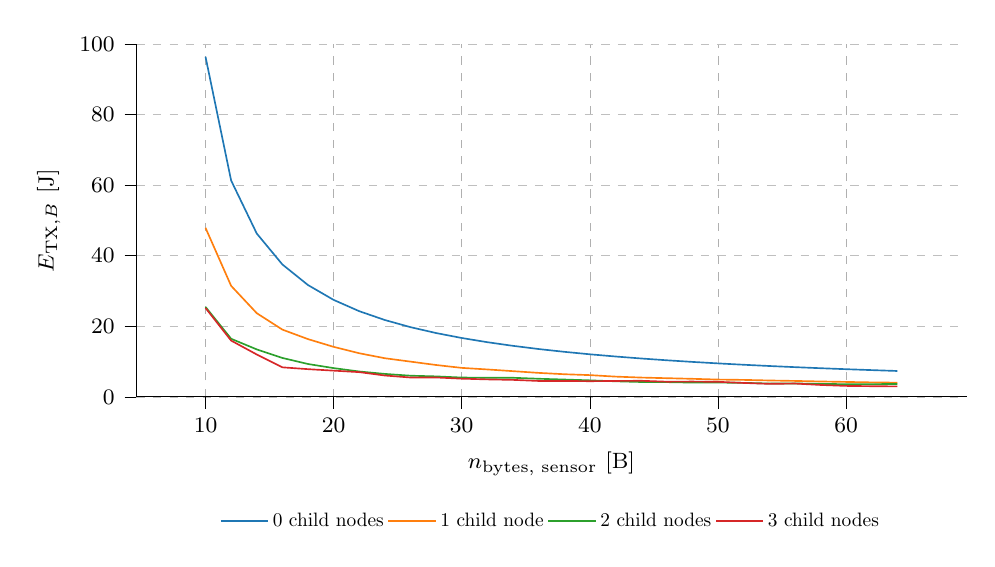
\begin{tikzpicture}

\definecolor{crimson2143940}{RGB}{214,39,40}
\definecolor{darkgray176}{RGB}{176,176,176}
\definecolor{darkorange25512714}{RGB}{255,127,14}
\definecolor{forestgreen4416044}{RGB}{44,160,44}
\definecolor{mediumpurple148103189}{RGB}{148,103,189}
\definecolor{sienna1408675}{RGB}{140,86,75}
\definecolor{steelblue31119180}{RGB}{31,119,180}


\begin{axis}[
    axis line style={black},
    axis lines* = {left},
    legend cell align={left},
    legend style={ at={(0.5,-0.3)},anchor=north, fill opacity=0.8, draw opacity=1, text opacity=1, draw=white!80.00000!black, %/tikz/column 2/.style={column sep=5pt}, /tikz/column 3/.style={column sep=5pt}
    },
    legend style={draw=none, nodes={scale=0.7, transform shape}},
    legend columns=4, 
    tick align=outside,
    tick pos=left,
    width = 1\linewidth,
    height=0.5\linewidth,
    x grid style={white!69.01960784313725!black},
    grid,
    grid style={help lines,color=gray!50, dashed},
    xtick style={color=black},
    %ylabel={energy\_per\_payload\_byte},
    ylabel={$E_{\text{TX},B}$ [J]},
    %xlabel={$T_a$ [\si{\minute}]},
    xlabel={$n_{\text{bytes, sensor}}$ [B]},
    ytick style={color=black},
    label style={font=\footnotesize},
    tick label style={font=\footnotesize, /pgf/number format/fixed},
    %ytick={0.0,0.1,0.2,0.3,0.4,5},
    %yticklabel={\pgfmathparse{\tick/60}$\pgfmathprintnumber{\pgfmathresult}$},
    %ytick={0, 180, 360, 540, 720, 900, 1080},
    %xticklabel={\pgfmathparse{(\tick/60)/30}$\pgfmathprintnumber{\pgfmathresult}$},
    clip=false,
    ymax=100,
    ymin=0
    ]
    


\addplot [semithick, steelblue31119180]
table {%
2 nan
4 nan
6 nan
8 nan
10 96.4109089782992
12 61.3178637826406
14 46.2954208643339
16 37.5259947811903
18 31.6898390021547
20 27.4830531525844
22 24.2830670587858
24 21.7796279243611
26 19.7569064782422
28 18.0885680878909
30 16.6867678092351
32 15.4939289321718
34 14.4638402519201
36 13.558713331028
38 12.7688664983217
40 12.0671888709391
42 11.4419896642999
44 10.8795560218392
46 10.3717172431416
48 9.91177526454337
50 9.48763868380214
52 9.10357051706712
54 8.75034299024043
56 8.42559291010138
58 8.1234569514943
60 7.84391471281999
62 7.58329924783773
64 7.33665985632679
};
\addlegendentry{0 child nodes}
\addplot [semithick, darkorange25512714]
table {%
2 nan
4 nan
6 nan
8 nan
10 47.9093528914338
12 31.4627544613783
14 23.7165023632884
16 19.0616974893504
18 16.3677744337652
20 14.1740074455262
22 12.3620745180918
24 10.9507096733628
26 9.99105470613179
28 9.03092037386809
30 8.21618208921837
32 7.77030881141955
34 7.28640245907269
36 6.80008453199627
38 6.41965032239291
40 6.16504948409908
42 5.74304939747145
44 5.47312638650469
46 5.29428787422656
48 5.11967602998673
50 4.90567641511894
52 4.81120271859789
54 4.64723085343549
56 4.51944323323616
58 4.36597514231445
60 4.23555423058481
62 4.10524687039339
64 4.02585637855389
};
\addlegendentry{1 child node}
\addplot [semithick, forestgreen4416044]
table {%
2 nan
4 nan
6 nan
8 nan
10 25.496469282876
12 16.4621683359588
14 13.4547516788679
16 11.0316292273386
18 9.31613854877005
20 8.15213541585441
22 7.19202763719996
24 6.50604988631577
26 6.00040312753238
28 5.80380833612591
30 5.47802702566212
32 5.42796637853115
34 5.41016212919466
36 5.13443754679501
38 4.91481355331174
40 4.68362247047423
42 4.41465454767239
44 4.21586070501474
46 4.1793833004835
48 4.04757257405861
50 4.05603563049337
52 3.96911540915444
54 3.78784042857381
56 3.80479145597749
58 3.68524939638035
60 3.58972863370585
62 3.61830062105307
64 3.6366082726892
};
\addlegendentry{2 child nodes}
\addplot [semithick, crimson2143940]
table {%
2 nan
4 nan
6 nan
8 nan
10 25.2008800485038
12 15.9501792595473
14 12.0117243561346
16 8.37442061415241
18 7.85236900607818
22 7.01129344831963
24 6.05647229260708
26 5.4868909863197
28 5.49384138292499
30 5.16029639316589
32 4.95310771485625
34 4.81641654414709
36 4.50896208671403
38 4.52041799999637
40 4.43805708800297
42 4.51267956263136
44 4.56230811118813
46 4.30181801858377
48 4.33878130743749
50 4.26903901445202
52 3.94391549379945
54 3.69032243294957
56 3.77852430498726
58 3.37709026090509
60 3.1074721069539
62 3.02531421554818
64 2.96492629551514
};
\addlegendentry{3 child nodes}
\end{axis}

\end{tikzpicture}

    \vspace{-0.7cm}
    \caption{Simulated transmit energy per byte ($E_{\text{TX}, B}$ across the \multihop network w.r.t. the data size of one sensor value ($n_\text{bytes, sensor}$).}
    \label{fig:}
\end{figure}
\begin{figure}[p]
    \centering
    % This file was created with tikzplotlib v0.10.1.
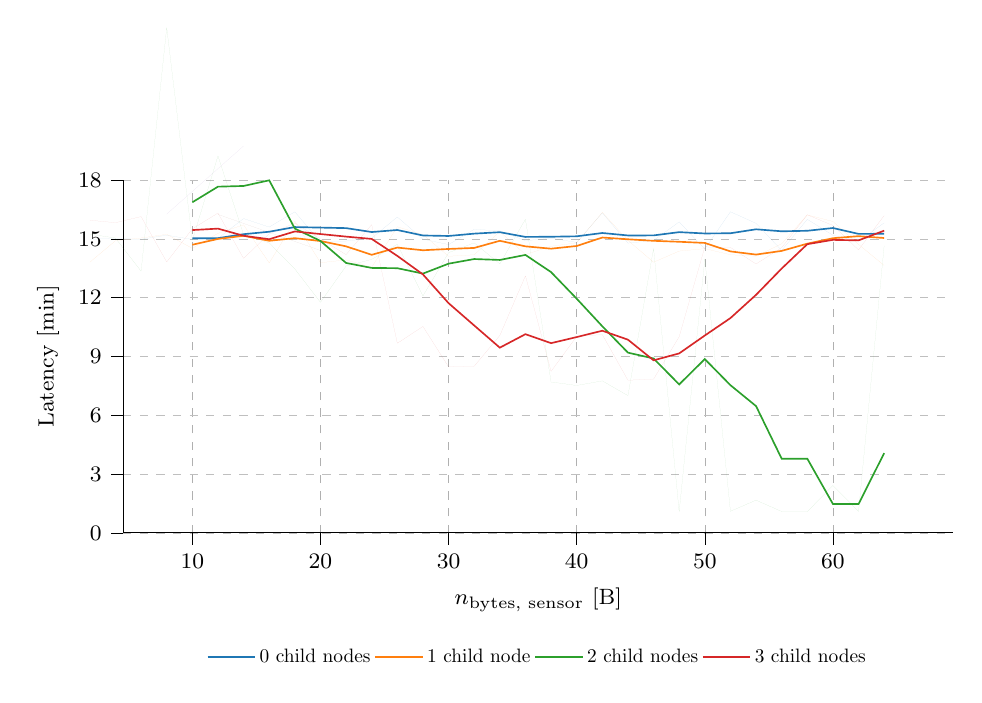
\begin{tikzpicture}

\definecolor{crimson2143940}{RGB}{214,39,40}
\definecolor{darkgray176}{RGB}{176,176,176}
\definecolor{darkorange25512714}{RGB}{255,127,14}
\definecolor{forestgreen4416044}{RGB}{44,160,44}
\definecolor{mediumpurple148103189}{RGB}{148,103,189}
\definecolor{sienna1408675}{RGB}{140,86,75}
\definecolor{steelblue31119180}{RGB}{31,119,180}

\begin{axis}[
    axis line style={black},
    axis lines* = {left},
    legend cell align={left},
    legend style={ at={(0.5,-0.3)},anchor=north, fill opacity=0.8, draw opacity=1, text opacity=1, draw=white!80.00000!black, %/tikz/column 2/.style={column sep=5pt}, /tikz/column 3/.style={column sep=5pt}
    },
    legend style={draw=none, nodes={scale=0.7, transform shape}},
    legend columns=4, 
    tick align=outside,
    tick pos=left,
    width = 1\linewidth,
    height=0.5\linewidth,
    x grid style={white!69.01960784313725!black},
    grid,
    grid style={help lines,color=gray!50, dashed},
    xtick style={color=black},
    %ylabel={energy\_per\_payload\_byte},
    ylabel={Latency [min]},
    %xlabel={$T_a$ [\si{\minute}]},
    xlabel={$n_{\text{bytes, sensor}}$ [B]},
    ytick style={color=black},
    label style={font=\footnotesize},
    tick label style={font=\footnotesize, /pgf/number format/fixed},
    %ytick={0.0,0.1,0.2,0.3,0.4,5},
    yticklabel={\pgfmathparse{\tick/60}$\pgfmathprintnumber{\pgfmathresult}$},
    ytick={0, 180, 360, 540, 720, 900, 1080},
    %xticklabel={\pgfmathparse{(\tick/60)/30}$\pgfmathprintnumber{\pgfmathresult}$},
    clip=false,
    ymax=1080,
    ymin=0
    ]
\path [fill=steelblue31119180, fill opacity=0.3]
(axis cs:2,899.057811618412)
--(axis cs:2,899.057811618412)
--(axis cs:4,900.838434285079)
--(axis cs:6,898.776010665966)
--(axis cs:8,911.296673522883)
--(axis cs:10,898.224243399412)
--(axis cs:12,901.403701454991)
--(axis cs:14,962.092243272962)
--(axis cs:16,936.105156000082)
--(axis cs:18,982.781672571271)
--(axis cs:20,890.069204571107)
--(axis cs:22,893.346898856822)
--(axis cs:24,902.338327999344)
--(axis cs:26,966.908253683608)
--(axis cs:28,899.11120590452)
--(axis cs:30,882.491157142677)
--(axis cs:32,929.069820761574)
--(axis cs:34,924.594224380495)
--(axis cs:36,894.381833714198)
--(axis cs:38,901.946961714324)
--(axis cs:40,889.124938857179)
--(axis cs:42,979.668249332587)
--(axis cs:44,887.039950485688)
--(axis cs:46,895.111129333501)
--(axis cs:48,951.960174416274)
--(axis cs:50,868.773717904934)
--(axis cs:52,982.999214980448)
--(axis cs:54,947.507978419097)
--(axis cs:56,864.685242285898)
--(axis cs:58,959.788099636572)
--(axis cs:60,910.936905894947)
--(axis cs:62,893.343964000208)
--(axis cs:64,948.860128000099)
--(axis cs:64,948.860128000099)
--(axis cs:64,948.860128000099)
--(axis cs:62,893.343964000208)
--(axis cs:60,910.936905894947)
--(axis cs:58,959.788099636572)
--(axis cs:56,864.685242285898)
--(axis cs:54,947.507978419097)
--(axis cs:52,982.999214980448)
--(axis cs:50,868.773717904934)
--(axis cs:48,951.960174416274)
--(axis cs:46,895.111129333501)
--(axis cs:44,887.039950485688)
--(axis cs:42,979.668249332587)
--(axis cs:40,889.124938857179)
--(axis cs:38,901.946961714324)
--(axis cs:36,894.381833714198)
--(axis cs:34,924.594224380495)
--(axis cs:32,929.069820761574)
--(axis cs:30,882.491157142677)
--(axis cs:28,899.11120590452)
--(axis cs:26,966.908253683608)
--(axis cs:24,902.338327999344)
--(axis cs:22,893.346898856822)
--(axis cs:20,890.069204571107)
--(axis cs:18,982.781672571271)
--(axis cs:16,936.105156000082)
--(axis cs:14,962.092243272962)
--(axis cs:12,901.403701454991)
--(axis cs:10,898.224243399412)
--(axis cs:8,911.296673522883)
--(axis cs:6,898.776010665966)
--(axis cs:4,900.838434285079)
--(axis cs:2,899.057811618412)
--cycle;

\path [fill=darkorange25512714, fill opacity=0.3]
(axis cs:2,828.479303999509)
--(axis cs:2,828.479303999509)
--(axis cs:4,894.242773999444)
--(axis cs:6,902.654579999191)
--(axis cs:8,913.883040799374)
--(axis cs:10,870.937043999391)
--(axis cs:12,916.881473999843)
--(axis cs:14,942.834026666638)
--(axis cs:16,826.128203999577)
--(axis cs:18,954.021904999967)
--(axis cs:20,827.022434400013)
--(axis cs:22,835.621434999953)
--(axis cs:24,813.038361843986)
--(axis cs:26,936.936693097645)
--(axis cs:28,913.143056000086)
--(axis cs:30,846.756268000082)
--(axis cs:32,851.335012000082)
--(axis cs:34,922.178930877903)
--(axis cs:36,852.102136000083)
--(axis cs:38,877.290228000086)
--(axis cs:40,887.858350877904)
--(axis cs:42,980.959478877912)
--(axis cs:44,895.497590877907)
--(axis cs:46,828.459292000084)
--(axis cs:48,862.607569031676)
--(axis cs:50,870.035030965802)
--(axis cs:52,851.455682965823)
--(axis cs:54,846.906337031664)
--(axis cs:56,884.858758965792)
--(axis cs:58,973.382823387588)
--(axis cs:60,953.267227387607)
--(axis cs:62,883.079819387606)
--(axis cs:64,818.484651387579)
--(axis cs:64,818.484651387579)
--(axis cs:64,818.484651387579)
--(axis cs:62,883.079819387606)
--(axis cs:60,953.267227387607)
--(axis cs:58,973.382823387588)
--(axis cs:56,884.858758965792)
--(axis cs:54,846.906337031664)
--(axis cs:52,851.455682965823)
--(axis cs:50,870.035030965802)
--(axis cs:48,862.607569031676)
--(axis cs:46,828.459292000084)
--(axis cs:44,895.497590877907)
--(axis cs:42,980.959478877912)
--(axis cs:40,887.858350877904)
--(axis cs:38,877.290228000086)
--(axis cs:36,852.102136000083)
--(axis cs:34,922.178930877903)
--(axis cs:32,851.335012000082)
--(axis cs:30,846.756268000082)
--(axis cs:28,913.143056000086)
--(axis cs:26,936.936693097645)
--(axis cs:24,813.038361843986)
--(axis cs:22,835.621434999953)
--(axis cs:20,827.022434400013)
--(axis cs:18,954.021904999967)
--(axis cs:16,826.128203999577)
--(axis cs:14,942.834026666638)
--(axis cs:12,916.881473999843)
--(axis cs:10,870.937043999391)
--(axis cs:8,913.883040799374)
--(axis cs:6,902.654579999191)
--(axis cs:4,894.242773999444)
--(axis cs:2,828.479303999509)
--cycle;

\path [fill=forestgreen4416044, fill opacity=0.3]
(axis cs:2,914.79525112773)
--(axis cs:2,914.79525112773)
--(axis cs:4,902.359557045651)
--(axis cs:6,801.079745845566)
--(axis cs:8,1546.42939899907)
--(axis cs:10,895.136296204612)
--(axis cs:12,1153.68899600014)
--(axis cs:14,913.170714027284)
--(axis cs:16,887.644176615329)
--(axis cs:18,807.857010338323)
--(axis cs:20,705.888984000132)
--(axis cs:22,816.88504233838)
--(axis cs:24,837.085792984441)
--(axis cs:26,883.296808000149)
--(axis cs:28,725.27234160021)
--(axis cs:30,857.75619200029)
--(axis cs:32,887.740748000263)
--(axis cs:34,823.364044000132)
--(axis cs:36,960.085240000171)
--(axis cs:38,461.952168000162)
--(axis cs:40,451.226052000154)
--(axis cs:42,465.324656000152)
--(axis cs:44,420.25596000014)
--(axis cs:46,870.690548000362)
--(axis cs:48,64.8713160001544)
--(axis cs:50,838.73268800038)
--(axis cs:52,66.1704240001127)
--(axis cs:54,100.179012000123)
--(axis cs:56,65.5066800001314)
--(axis cs:58,65.2283080001553)
--(axis cs:60,145.248948000138)
--(axis cs:62,65.7682920001107)
--(axis cs:64,879.342872000343)
--(axis cs:64,879.342872000343)
--(axis cs:64,879.342872000343)
--(axis cs:62,65.7682920001107)
--(axis cs:60,145.248948000138)
--(axis cs:58,65.2283080001553)
--(axis cs:56,65.5066800001314)
--(axis cs:54,100.179012000123)
--(axis cs:52,66.1704240001127)
--(axis cs:50,838.73268800038)
--(axis cs:48,64.8713160001544)
--(axis cs:46,870.690548000362)
--(axis cs:44,420.25596000014)
--(axis cs:42,465.324656000152)
--(axis cs:40,451.226052000154)
--(axis cs:38,461.952168000162)
--(axis cs:36,960.085240000171)
--(axis cs:34,823.364044000132)
--(axis cs:32,887.740748000263)
--(axis cs:30,857.75619200029)
--(axis cs:28,725.27234160021)
--(axis cs:26,883.296808000149)
--(axis cs:24,837.085792984441)
--(axis cs:22,816.88504233838)
--(axis cs:20,705.888984000132)
--(axis cs:18,807.857010338323)
--(axis cs:16,887.644176615329)
--(axis cs:14,913.170714027284)
--(axis cs:12,1153.68899600014)
--(axis cs:10,895.136296204612)
--(axis cs:8,1546.42939899907)
--(axis cs:6,801.079745845566)
--(axis cs:4,902.359557045651)
--(axis cs:2,914.79525112773)
--cycle;

\path [fill=crimson2143940, fill opacity=0.3]
(axis cs:2,957.020099352044)
--(axis cs:2,957.020099352044)
--(axis cs:4,949.577278146853)
--(axis cs:6,968.174510146873)
--(axis cs:8,829.38135906826)
--(axis cs:10,930.590820293596)
--(axis cs:12,978.934868000196)
--(axis cs:14,840.232838131361)
--(axis cs:16,915.382340293606)
--(axis cs:18,948.196672293609)
--(axis cs:22,851.635296293596)
--(axis cs:24,943.67792829362)
--(axis cs:26,580.454396000295)
--(axis cs:28,631.902456000285)
--(axis cs:30,508.187152000175)
--(axis cs:32,510.165740000194)
--(axis cs:34,604.16942000038)
--(axis cs:36,786.912188000383)
--(axis cs:38,494.468368000187)
--(axis cs:40,601.490636000301)
--(axis cs:42,607.072976000281)
--(axis cs:44,467.346904000256)
--(axis cs:46,470.641332000295)
--(axis cs:48,600.566604000201)
--(axis cs:50,875.285829934232)
--(axis cs:52,873.767581934233)
--(axis cs:54,823.131424000087)
--(axis cs:56,873.014457934235)
--(axis cs:58,973.73850635603)
--(axis cs:60,940.924174356028)
--(axis cs:62,866.146022356023)
--(axis cs:64,971.457134356032)
--(axis cs:64,971.457134356032)
--(axis cs:64,971.457134356032)
--(axis cs:62,866.146022356023)
--(axis cs:60,940.924174356028)
--(axis cs:58,973.73850635603)
--(axis cs:56,873.014457934235)
--(axis cs:54,823.131424000087)
--(axis cs:52,873.767581934233)
--(axis cs:50,875.285829934232)
--(axis cs:48,600.566604000201)
--(axis cs:46,470.641332000295)
--(axis cs:44,467.346904000256)
--(axis cs:42,607.072976000281)
--(axis cs:40,601.490636000301)
--(axis cs:38,494.468368000187)
--(axis cs:36,786.912188000383)
--(axis cs:34,604.16942000038)
--(axis cs:32,510.165740000194)
--(axis cs:30,508.187152000175)
--(axis cs:28,631.902456000285)
--(axis cs:26,580.454396000295)
--(axis cs:24,943.67792829362)
--(axis cs:22,851.635296293596)
--(axis cs:18,948.196672293609)
--(axis cs:16,915.382340293606)
--(axis cs:14,840.232838131361)
--(axis cs:12,978.934868000196)
--(axis cs:10,930.590820293596)
--(axis cs:8,829.38135906826)
--(axis cs:6,968.174510146873)
--(axis cs:4,949.577278146853)
--(axis cs:2,957.020099352044)
--cycle;

\path [fill=mediumpurple148103189, fill opacity=0.3]
(axis cs:8,975.742992000169)
--(axis cs:8,975.742992000169)
--(axis cs:14,1184.37724800016)
--(axis cs:14,1184.37724800016)
--(axis cs:14,1184.37724800016)
--(axis cs:8,975.742992000169)
--cycle;

\path [fill=sienna1408675, fill opacity=0.3]
(axis cs:12,974.882012293606)
--(axis cs:12,974.882012293606)
--(axis cs:20,864.608404293597)
--(axis cs:20,864.608404293597)
--(axis cs:20,864.608404293597)
--(axis cs:12,974.882012293606)
--cycle;

\addplot [semithick, steelblue31119180]
table {%
2 nan
4 nan
6 nan
8 nan
10 901.63863469835
12 902.107812665666
14 914.358574463243
16 921.824403530066
18 936.121403339744
20 934.490395574083
22 932.879035054449
24 920.928251999725
26 927.08887153643
28 910.35477820308
30 908.839168717394
32 915.983753098344
34 920.434932374575
36 905.929648380693
38 906.496799542654
40 907.823555885554
42 917.943241599757
44 910.432386820795
46 910.578245944656
48 920.580888485046
50 916.510644294597
52 917.176837424169
54 929.270443010851
56 923.18526560133
58 924.75085064539
60 933.183488243393
62 915.252438047345
64 915.522867963545
};
\addlegendentry{0 child nodes}
\addplot [semithick, darkorange25512714]
table {%
2 nan
4 nan
6 nan
8 nan
10 882.039348559382
12 899.719782559449
14 909.438033092887
16 894.132757892965
18 902.160530733083
20 893.377608813208
22 877.12560101323
24 851.166468048699
26 873.328165868313
28 865.152396068337
30 869.09916278835
32 872.241878188376
34 894.06999199516
36 877.103080575647
38 869.932514975647
40 878.152931551212
42 904.077824926778
44 898.741556926778
46 894.012988126779
48 891.076456333097
50 887.511792350676
52 861.611033168258
54 851.89278239901
56 863.172675792151
58 885.327726663334
60 901.974165947695
62 908.298993232051
64 902.614656103234
};
\addlegendentry{1 child node}
\addplot [semithick, forestgreen4416044]
table {%
2 nan
4 nan
6 nan
8 nan
10 1011.96004984452
12 1059.73879881901
14 1061.90103021533
16 1079.21391636929
18 931.499438637137
20 893.649976196241
22 826.28918546389
24 811.072201255321
26 810.202727532285
28 793.685793784662
30 824.059235384694
32 838.230376517071
34 835.486026720209
36 850.843713120213
38 798.179678400203
40 716.873650400176
42 632.390432000154
44 551.768815200156
46 533.889876800194
48 454.473706400192
50 531.975033600238
52 452.14418720023
54 388.128797600226
56 227.09202400018
58 227.163422400181
60 88.4666744001321
62 88.3862480001317
64 244.219020000176
};
\addlegendentry{2 child nodes}
\addplot [semithick, crimson2143940]
table {%
2 nan
4 nan
6 nan
8 nan
10 926.948813401525
12 931.331767131156
14 909.462879128057
16 898.904445157404
18 922.667507802473
22 906.876403002473
24 899.825015061158
26 847.869326634945
28 791.173349776281
30 703.171445717594
32 634.877534458914
34 566.975832800266
36 608.267391200284
38 580.780573600264
40 599.441270400289
42 618.822717600307
44 591.458214400282
46 528.204043200264
48 549.423690400267
50 604.182729187053
52 657.521650373843
54 728.678554373809
56 809.153179560598
58 883.787560031764
60 896.915228916123
62 895.390917000481
64 925.05605907167
};
\addlegendentry{3 child nodes}
\end{axis}

\end{tikzpicture}

    \vspace{-0.7cm}
    \caption{Simulated latency of sensor readings across the \multihop network w.r.t. the data size of one sensor value ($n_\text{bytes, sensor}$).}
    \label{fig:}
\end{figure}

\end{document}
